
\documentclass[quali, eng]{ita}    % ITA.cls based on standard book.cls 
%\usepackage[brazilian]{babel}
\usepackage{ae}
\usepackage{graphicx}
\usepackage{epsfig}
\usepackage{amsmath}
\usepackage{amssymb} 
\usepackage{multirow}
\usepackage{float}
\usepackage{color,xcolor,ucs}
\usepackage{hyperref}
\usepackage{pgfgantt}
\usepackage{pdflscape}
\usepackage{multicol}
\usepackage{enumitem}
\usepackage{todonotes}
\usepackage{subcaption}
\usepackage{mathtools}
\usepackage{nicefrac}

\usepackage{algorithm}
\usepackage{algorithmicx}
\usepackage[noend]{algpseudocode}

\makeatletter
\def\BState{\State\hskip-\ALG@thistlm}
\makeatother

\newcommand{\argmin}{\arg\,\min} 

\newtheorem{defn}{Definition}%[section]
%++++++++++++++++++++++++++++++++++++++++++++++++++++++++++++++++++++++++++++++
% Espacamento padrao de todo o documento
%++++++++++++++++++++++++++++++++++++++++++++++++++++++++++++++++++++++++++++++
\onehalfspacing

%singlespacing Para um espacamento simples
%onehalfspacing Para um espacamento de 1,5
%doublespacing Para um espacamento duplo

%++++++++++++++++++++++++++++++++++++++++++++++++++++++++++++++++++++++++++++++
\course{Electronic and Computer Engineering} 
\area{Informatics} 

% Autor do trabalho: Nome Sobrenome
\authorgender{masc}                    
\author{N\'{i}colas Pereira}{Borges}
\itaauthoraddress{Av. Cidade Jardim, 679}{12.233-066}{S\~{a}o Jos\'{e} dos Campos--SP}

% Titulo da Tese/Dissertacao

%\title{Improving stealth in collaborative UAV networks using a combined control law approach}
\title{Cooperative path planning approach to increase stealthiness in multidepot visiting applications}
\title{Dynamic Route Optimization for Drones in Denied Environment}


% Orientador
\advisorgender{masc}                    % masc ou fem
\advisor{Prof.~Dr.}{Carlos Henrique Costa Ribeiro}{ITA}

\coadvisorgender{fem}									% masc ou fem
\coadvisor{Dr$^\textnormal{a}$.}{Cinara Guellner Ghedini}{ITA}

% Pro-reitor da Pos-graduacao
\bossgender{masc}											
\boss{Prof.~Dr.}{Pedro Teixeira Lacava}

% Palavras-Chaves informadas pela Biblioteca -> utilizada na CIP
\kwcip{Stealth, unmanned aerial vehicles, multi-robot systems}


% membros da banca examinadora
\examiner{Prof. Dr.}{}{Chairperson}{ITA}
\examiner{Prof$^\textnormal{a}$. Dr$^\textnormal{a}$.}{}{Internal Member}{ITA}
\examiner{Prof$^\textnormal{a}$. Dr$^\textnormal{a}$.}{}{External Member}{}
%\examiner{Prof. Dr.}{Marcos Gon\c{c}alves Quiles}{}{UNIFESP}

% Data da defesa (mes em maiusculo, se trabalho em ingles, e minusculo se trabalho em portugues) 
\date{09}{September}{2019}

% Glossario
\makeglossary
\frontmatter

\begin{document}
% Folha de Rosto e Capa para o caso do TG
\maketitle

%\begin{itadedication}

%\end{itadedication}

% Agradecimentos
%\begin{itathanks}
%First off all, I want to thanks my advisor Prof. Carlos Henrique Costa Ribeiro for his precious support during this research. I am grateful for the patience and comprehension in the face of adversity that occurred throughout the program.

My special thanks to my co-advisor Cinara Guellner Ghedini not only for the outstanding support during this research and the encouragement during the program, but mainly for the friendship. 

I would also like to thank professors Carlos Henrique Quartucci Forster, Neusa Maria Franco de Oliveira and Lilian Berton for their valuable contribution as member of the Thesis Committee.

I would like to thank my family for supporting me in all my pursuits, specially to my brother Nataniel for the meticulous review of my thesis.

My special thanks to professors Anita Maria da Rocha Fernandes and Edson Tadeu Bez for the recommendation letters and for supporting me all the time. I would also like to thanks Jorge Destri Jr by its contribution by reviewing my master thesis and for the support during this research. Moreover, thanks to Diogo Andrei Benvenutti for the support in optimizing my source code in C++ and for encouragement. I am grateful to Caroline Mazzuco Furlan for the friendship and the support on mathematics aspects of the model. 

During this work, many friends and colleagues were very important. It is not possible to mention all, however some of these deserve to be highlighted. Thanks to my friends from Santa Catarina: Vitor Whays, Daniel Adriano, Rejane Araujo, Kerle Loffy, Ricardo Giordani and Leonardo Fenill. To my colleagues from ITA: Rene Esteves, Strauss Cunha, Rosana Teixeira, Mayara Moraes, Lucas Povoa, Jo{\~a}o Siles, Lais Siles and Paulo Diego Barbosa. In addition, thanks to my colleagues of Brazilian Air Force, especially to James de Castro Martins, Silvio Assun\c{c}ao and Ricardo Silva de Oliveira. 

I gratefully acknowledge CNPQ (Conselho Nacional de Desenvolvimento Cient{\'i}fico e Tecnol{\'o}gico) for the financial support.
%\end{itathanks}

% Epigrafe
\thispagestyle{empty}
\ifhyperref\pdfbookmark[0]{\nameepigraphe}{epigrafe}\fi
\begin{flushright}
\begin{spacing}{1}
%\mbox{}\vfill
%{\sffamily\itshape
%``The chance you got comes never twice. \\ Do your best, and do it right. \\Time will come but don't you hide. \\
%You are on your way.''\\}
%--- \textsc{Roland Grapow}
\end{spacing}
\end{flushright}

% Resumo
\begin{abstract}
\noindent
\input{Cap0/resumo}
\end{abstract}

% Abstract
\begin{englishabstract}
\noindent
\input{Cap0/abstract}
\end{englishabstract}

% Lista de figuras
\listoffigures %opcional

% Lista de tabelas
%\listoftables %opcional

% Lista de abreviaturas
\listofabbreviations
\begin{longtable}{ll}
UAV & Unmanned Aerial Vehicle\\

\end{longtable}

 %opcional

% Lista de simbolos
%\listofsymbols
%\begin{longtable}{ll}
%$UAV$ & Unmanned Aerial Vehicle\\
\end{longtable}

 %opcional


% Sumario
\tableofcontents

\mainmatter
% Os capitulos comecam aqui

\chapter{Introduction} \label{chap:1}
\section{Motivation}

Unmanned aerial vehicles (UAVs), commonly known as a drones, are replacing human pilots in potentially dangerous military missions. They are frequently deployed in missions of destroying enemy forces in denied environments. \cite{westra_2009, kacena1995}. One of the most reported cases in the beginning of 2020, regarding UAV's missions in military context, was the death o Iranian General Qasem Soleimani by an American UAV \cite{sarker_2020}. Another well known case was when the US special forces raided the safe-house of Osama Bin Laden in 2011 and caught him completely by surprise. In this mission, the UAVs were used to evade the Pakistani radar \cite{drew_2011}.

Due to the benefits of exploiting the surprise factor of monitored environments with aerial platforms, the use of stealth approaches becomes essential for mission success, because it allows missions to be conducted in proximity of threat radars and enemy air defences, by minimizing the signature of the aircraft, i.e., the traces left by the aircraft that can be used to detect it. According to Kacena \cite{kacena1995} stealth can be defined as a combination of techniques and technologies that aims at increasing the enemy's difficulty in detecting, tracking, guiding or predicting an object's future positions in space.

Regarding security, the use of manned airplanes for some missions may be risky, as it may endanger the life of the pilots \cite{venancio_2007}. On the other hand, UAVs can be sent into hostile areas with no risk to the lives of pilots \cite{mod_2011, foust_2012}. There are two classes of UAVs: non-autonomous and autonomous. For missions adopting non-autonomous UAVs, i.e., vehicles remotely controlled by a human operator, the mission success is directly related to the operator skills and to the endurance of the operator. Autonomous UAVs can perform actions such as detection, identification, targeting and engagement of an enemy faster than their non-autonomous counterparts \cite{bellamy_2015}.

Besides attack missions, UAVs can also be provide supply, maintenance, health services, and other services required by the soldiers of combat units to continue their missions in combat. According to \citeauthor{aeronautica_2012}, this kind of application is named Combat Service Support \cite{aeronautica_2012}. They can be used to deliver of combat supplies from a physical base or a vehicle to personnel engaged in combat operations or even reconnaissance missions. Examples of applications can include military equipment or even ambulance UAVs that deliver medicines, immunizations, and blood samples \cite{amukele_2017}. 

This kind of application is strong related with Vehicle Routing Problems (VRPs), because it is necessary to trace the route of each UAV. Also, depending on the  route, the whole mission can be compromised. According to \cite{toth_2002}, VRPs are characterized by the determination of the optimal set of routes to be performed by a fleet of vehicles to serve a given set of customers, and it is one of the most important, and studied, combinatorial optimization problems. According to \cite{thornton_2018}, current modes of drone-routing in military operations primarily involve the use of crewed supply vehicles and air drops, however the use of autonomous UAVs can provide several benefits.

In many applications, not all information about the problem instance is known prior. Considering delivery application, the most common dynamic events are the arrival of new customer requests. On the other hand, in military missions, it is necessary to consider that enemies can be discovered during the mission. Then, when a threat is detected, the UAVs need to react to the enemy in order to increase the probability of mission succeed  \cite{zhou_2018}. Also, the adjustment of the planned solution according to the plan in execution is another crucial factor and can be performed with different updating strategies. The class of vehicle-routing problem that modelling dynamic scenarios is named Dynamic Vehicle-Routing Problems (DVRP), also referred to as real-time or online VRP \cite{ritzinger_2016}. 

The Dynamic Vehicle Routing problem performed by several autonomous UAVs, considering an hostile environment, monitored by radars has not deeply studied in literature. We are assuming as the dynamic factor the unknown presence of enemy (enemy radars). The problem consists in visiting several waypoints and then return to the base, while minimizing the total flight time. Also, we will consider a time window, since UAVs have limited battery. The UAVs do not know about the presence of threats prior. Thus, as long as they detect a threat, they need to react in order to evade it, while perform stealth policies to reduce the exposure to the enemy. At this moment, the route need to be dynamically optimized, considering the presence of the enemy.  Figure \ref{fig:scenario} shows the proposed scenario. In this figure, the scenario is composed of 3 UAVs, 6 waypoints (represented by soldiers) an 3 threats. This scenario consider that 3 UAVs were not discovered yet by UAVs. However it is possible to see problem of static vehicle routing. The paths passes trough all the radars.

\begin{figure}[h!]
    \centering
    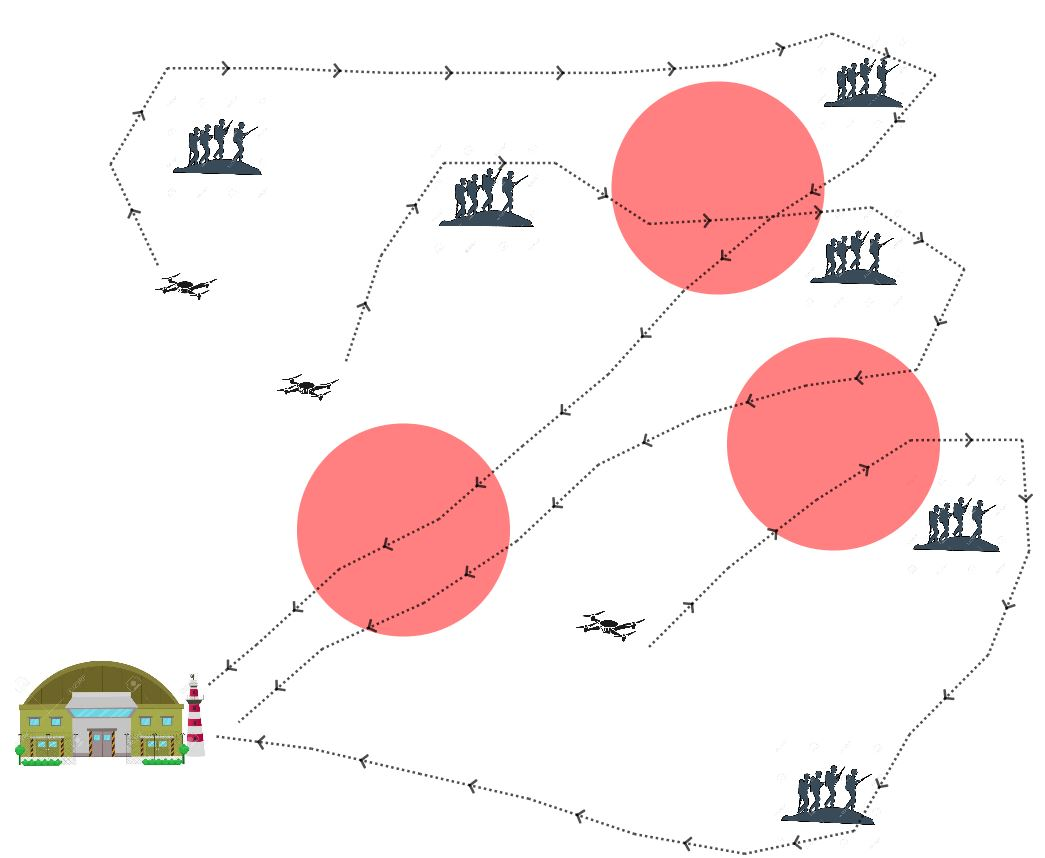
\includegraphics[width=0.6\textwidth]{Figures/scenario.JPG}
    \caption{An instance of the proposed scenario.}
    \label{fig:scenario}
\end{figure}


In this context, modelling a dynamic route optimization, considering multiple autonomous UAVs, assuming as the dynamic factor the unknown presence of enemy still is an open issue. The goal of this thesis is to propose a model that increases the UAVs stealthiness dynamically. This kind of problem can be considered as a DVRP. However, traditional DVRPs do not consider military operations and the impact of the stealthiness to the mission success.

\section{Objectives}

The goal of this thesis is to propose a model that increases stealth of autonomous UAVs during multi-target visiting missions. More specifically, it defines a model to reduce UAVs' exposure to threats through a combination of threat detection, path planning and dynamic route planning mechanisms.

We aim to assess the impact of different levels of hostility, regardless of UAVs stealth. Besides the reduction of flight time, the UAVs will try to increase their reliability, by adopting policies to detect and avoid threats. The evaluation of the model will consider three aspects: total flight time, stealth level of UAVs and the fraction of UAVs hit by the enemy.

\section{Contributions}

In this work we make the following contributions:

\begin{itemize}

    \item A review of logistical support missions in military environment. The result will be the identifications of  concepts, applications and peculiarities of logistics support missions to design simulation scenarios which correctly model their behavior.
    
    \item A review of state of art in DVRP. The result will be the study of models, that consider single and multiple UAVs, for the goods delivery. Moreover, we can select and evaluate appropriate models to be implemented in our scenario.
    
    \item We demonstrate how the coordinated use of multiple autonomous UAVs to perform routing affects the overall delivery time for logistical support missions, as well as the reliability of the delivery process. Our approach performs a route optimization while taking into account payload capacity and battery life.
    
    \item We demonstrate how the coordinate use of multiple UAVs can benefit logistical support in military operations. Our approach performs a Dynamic Route Optimization to re-plan the trajectory of UAVs when threats are discovered. Thi while trying to minimize the total flight time.
    
\end{itemize}


\section{Outline}
%The remaining of this work is organized as follows. In Chapter \ref{chap:2} we present the background of the research, addressing the way that military missions are performed and the importance of UAVs for missions and some of their characteristics. In addition, the stealth concept is described, relating its application to military missions performed by UAVs.

%In chapter \ref{chap:3} we present the related work of this research, emphasizing the characteristics of the stealth approach used in this work.

%Chapter \ref{chap:4} presents the computational model for improving stealthiness in collaborative UAV networks. The mechanism for detecting the threats and the stealth policy of UAVs to reduce the exposure to threats is detailed, as well as the way the UAVs move through the combination of control laws for path planning, coverage area improvement, connectivity robustness and maintenance.

%In chapter \ref{chap:5} we present the performed experiments to show the feasibility of our model, and a discussion about the achieved results for varying number of UAVs in the network and hostility level of the scenarios.

%Finally, Chapter \ref{chap:6} presents the conclusions, final considerations and proposals for extensions.




\chapter{Background}\label{chap:2}
\section{Military Operations}

In 2011, the US special forces who raided the safe house of Osama Bin Laden caught him completely by surprise by using drones to evade the Pakistani radar [5]

The way military missions performed by aircraft are carried out continuously changes. Nowadays, environments are being monitored by different types of electromagnetic devices, making necessary to adopt new approaches to take advantage from the opponent by using the surprise factor \cite{exercito_2009, kacena1995}. 

In addition to radars, there are other kinds of treats, whose purpose is to destroy an aircraft, such as Fire-Control Radars (FCR). According to Berglund \cite{berglund_2001}, the problem of penetrating enemy air defences is a concern for most sorts of aerial vehicles. Long range strike missiles are likely to be used against the enemy air defences in conjunction with other components, such as EW. The traditional approach for defence penetration is to attempt to avoid the detection of an aircraft until it is too late for the defences to react effectively.

Considering military operations performed in hostile environments, according to \citeauthor{aeronautica_2012} \cite{aeronautica_2012}, some of missions performed by aircraft are:
\begin{itemize}
    \item \textbf{Direct Action:} to neutralize enemies for strategic or operational purposes. This action is performed on hostile environment or area controlled by the enemies. 
    \item \textbf{Approximate Air Support:} to detect, identify and neutralize enemy surface forces that are in direct contact with friendly surface forces.
    \item \textbf{Air Reconnaissance:} to gather specific data onto enemy forces and areas of interest.
    \item \textbf{Scan:} to detect, identify and neutralize enemy forces in areas of interest.
    \item \textbf{Combat Service Support:}  to provide supply, maintenance, transportation, health services, and other services required by the soldiers of combat units to continue their missions in combat
\end{itemize}

The focus of this work relies on the Combat Service Support missions. This kind of missions must address highly uncertain conditions. While perfect forecasts are rarely possible, forecast models can reduce uncertainty about what supplies or services will be needed, where and when they will be needed, or the best way to provide them. In this context, the use of stealth approaches becomes essential. The expression stealth can be defined as a combination of techniques and technologies that aims at increasing the enemy's difficulty in detecting, tracking, guiding or predicting an object's future position in space by reducing the aircraft signature \cite{kacena1995}. Singh \cite{singh_2015} describes some of these factor, as follows:

\begin{itemize}
    \item Acoustic: The acoustic signatures of an aircraft are due to the aerodynamic noise from its vertices, wings, rotors, propellers and engines. The intensity of noise is proportional to the wingspan loading and speed. Reduction of such signature by coating the engine with sound-absorptive materials contributes to acoustic stealth.
    \item Optical: The optical signature of an aircraft is related to its size, shape and contrast with the background. The background luminance also depends upon the atmospheric conditions and the target position with respect to the sun. The surface-texture of the aircraft is other factor that impacts the optical signature.
    \item Thermal: The thermal signatures are due to the heat generated by the aircraft engines jets, propellers and rotors. The exhaust heat of the aircraft can be prevented by travelling towards the ground. Moreover, low-emissive materials can be used to avoid radiation. 
    \item Radar: The radar signatures are related to the radio frequency emissions from the aircraft. They can be reduced by either applying radar absorbent material coatings or shaping the aircraft. 
\end{itemize}

%The aircraft signature can be categorized as active or passive \cite{westra_2009}. According to \citeauthor{westra_2009} \cite{westra_2009}, an active signature consists in all the observable emissions from a stealth platform. On the other hand, the passive signatures can be defined as all the observable emissions from a stealth platform that require external illumination. In terms of nomenclature, the active signature reduction methods are commonly called low probability of interception (LPI), while passive signature reduction techniques are often called low observable (LO) \cite{westra_2009, lynch_2004}. 

In terms of techniques, it is possible to reduce the airplane signature with simple approaches, such as using natural hiding places provided by the environment, such as clouds and darkness \cite{haffa_2002}. In addition, radio or radar signals transmitted by an aircraft can also be used to detect an aircraft's position, therefore, techniques to decrease the probability of intercepting those signals, such as flying with radars turned off, using electronic pulses that do not exceed the range of the threat, and using frequency-hopping radios and radars to deny electromagnetic detection are all possible stealth mechanisms\cite{haffa_2002, friedman_2010}.

Aircrafts can be equipped with different sensors and radars. Regarding stealth, an active approach to detect a threat presence can expose aircrafts to passive enemy radars. Moreover, it is highly likely that an aircraft radar will have a detection range larger than an enemy vigilance radar, therefore it would be detected in advance. Due to this situation, the detection of the threats occurs passively on hostile environments. One equipment applied for this purpose is the Radar Warning Receiver (RWR), designed to detect radars as part of the process of protecting the target against those radars. It must detect a wide range of radar signals, which can come from any direction \cite{adamy2004}. The RWR has been used successfully by modern combat aircraft, such as the F-16, for many years \cite{brownlow_2008}. Regarding UAVs, tests using RWR on Predator B/MQ-9 Reaper Block 5 were successfully conducted on April 2017, allowing UAVs to operate in the proximity of threat radars and enemy air defenses \cite{osborn_2017}. 
  
  
During the last decades, manned airplanes were used for military missions. However, the number of applications relying on UAVs has significantly increased, since they are capable of carrying out missions that are too dangerous or difficult for humans \cite{mod_2011}. According to Jentsch \cite{jentsch_2016}, on future battle spaces each service and each ally will have its own set of aerial and ground uninhabited system with increasing levels of machine intelligence. In terms of real-world applications, to augment the capabilities of ground and air forces the U.S. military have developed several UAVs to work in conjunction with human pilots, thus enhancing their surveillance and combat capabilities \cite{mouloua_2001}. 

Considering that Combat Service Support is strong related to delivery systems, the use of autonomous drones can be promising. Drone delivery is one of the emerging areas of drone applications. These types of applications are very popular today because large companies have adopted this delivery system. For instance, the automation of Amazon package delivery enhances customer service by being able to provide rapid package delivery. UPS, Google and other European delivery services are also experimenting with delivery drones \cite{mack_2018}.


\section{Unmanned Aerial Vehicles}

The U.S. Department of Defense \cite{staff_2001} defines an unmanned aerial vehicle as a powered aerial vehicle that does not carry a human operator, uses aerodynamic forces to provide vehicle lift, can fly autonomously or be piloted remotely, can be expendable or recoverable, and can carry a lethal or non-lethal payload. UAVs can perform missions unconstrained by shift schedules or human endurance, conducting more surveillance and collecting more information than humans. Moreover, UAVs can execute a targeted strike with precision \cite{foust_2012}. 

UAVs have been used successfully for military purposes -- mainly reconnaissance -- since the 1950s \cite{sullivan_2005}. The Iraq war shifted the usage from strict reconnaissance to key weapon system performing many roles that are central to the operations \cite{fahlstrom_2012}. Currently, UAVs are essential for diverse military applications and can be categorized into fixed-wing and rotatory-wing (e.g. helicopters). Both categories are often used in military operations. Some UAVs weigh hundreds or even thousands of pounds and can fly more than 6000 feet while others, named small or micro UAVs, weigh less than 10 pounds and fly usually under 1,000 feet \cite{chao_2007}.

UAVs can be classified into groups based on its size, Maximum Gross Takeoff Weight (MGTW), Normal Operating Altitude (NOA) and Airspeed \cite{dempsey_2010}. Table \ref{tab:CategoryOfUAVs} shows the classification of UAVs based on these criteria. Notice that if an UAV has even one characteristic of the next level, it is classified in that level.

\begin{table}[hbt]
\centering
\caption{Categories of UAVs. Adapted from \cite{dempsey_2010}.}
\label{tab:CategoryOfUAVs}
\begin{tabular}{lllll}
\hline
Category & Size & MGTW (lbs) & NOA (ft) & Airspeed (knots) \\
\hline
Group 1  & Small   & 0-20                               & \textless1,200 Above Ground Level & \textless100     \\
Group 2  & Medium  & 21-55                              & \textless3,500                    & \textless250     \\
Group 3  & Large   & \textless1320                      & \textless18,000 Mean Sea Level    & \textless250     \\
Group 4  & Larger  & \textgreater1320                   & \textless18,000 Mean Sea Level    & Any airspeed     \\
Group 5  & Largest & \textgreater1320                   & \textgreater18,000                & Any airspeed  \\  
\hline
\end{tabular}
\end{table}

The majority of UAVs are designed for intelligence, surveillance and reconnaissance purposes. However, some UAVs are larger and armed and can more accurately be described as unmanned combat aerial vehicles (UCAVs) \cite{mayer_2015}. According to Wang \cite{wang_2012}, this is one of the inevitable trends of the modern aerial weapon equipment owing to its potential to perform dangerous, repetitive tasks in remote and hazardous environments. Research on UCAV directly affects battle effectiveness of the air force and is a fundamental field of research for the safeness of a nation \cite{wang_2012}. 

There are two classes of UAVs: non-autonomous and autonomous. Non-autonomous UAVs are remotely controlled by humans, and autonomous are capable of processing higher level intent and direction. From this understanding and its perception of its environment, such a system is able to take appropriate actions to bring about a desired state, and is capable of deciding a course of action, from a number of alternatives faster than non-autonomous counterparts, without depending on human oversight and control \cite{mod_2011, bellamy_2015}.

\section{Vehicle Routing problem}

Vehicle Routing Problem was first proposed by Dantzig and Ramsar 1959, and is mainly used to solve the transport route optimization problem: Atlanta's refinery problem. The subject quickly attracted the attention of experts and scholars, such as operations research, management, computer, graph theory, and proved to be widely used in transportation system, logistics distribution system and express delivery system. After several decades of development, the vehicle routing problem has become an important part of logistics management research, and is classified as the general term for such a type of problem: by a number of vehicles from one or more warehouses to multiple geographic On the distribution of customers, how to arrange the vehicle and its route to the total distribution costs can be minimized. 

Then, in theory, the VRP problem is defined as: organizing a series of loading and unloading points, as well as the corresponding traffic line organization, so that vehicles can be ordered through them. That is, to achieve the objectives and solve certain problems (such as shortest distance, minimum cost, time limit) under certain constraints (goods demand, delivery, delivery time,
vehicle capacity constraints, travel restrictions, time constraints, etc.)

VRP problems have a variety of classification methods and, for different classification methods, also have different corresponding models and algorithms. However, no matter how complex the model of the algorithm, common constraints in the discussion of VRP problem is the same capacity constraints [3]:

\begin{itemize}
    \item \textbf{Capacity constraints:} regardless of which vehicle, it should be less than the total path of the vehicle load capacity. 
    \item \textbf{Priority constraints:} leads to the priority of the vehicle to constrain the path problem.
    \item \textbf{Vehicle constraints:} leads to multi-vehicle vehicle routing problem.
    \item \textbf{Time window constraints:} including hard time window and soft time window constraints. The vehicle routing problem with time window.
    \item \textbf{Compatibility constraints:} leads to compatibility constraints of the vehicle routing problem.
    \item \textbf{Random demand:} leads to a random demand for the vehicle routing problem.
    \item \textbf{Multi-transport center:} leads to a multi-transport vehicle routing problem.
    \item \textbf{Return transport:} leads to a return route with the vehicle routing problem.
    \item \textbf{Vehicle speed changes with time:} with time, leads to the vehicle speed with time changes in vehicle routing problem
\end{itemize}

\subsection{Static Vehicle Routing problem}

\subsection{Dynamic Vehicle Routing problem}

The dynamic vehicle routing problem calls for online algorithms that work in real-time since the immediate requests should be served, if possible. As conventional static vehicle routing problems are NP hard, it is not always possible to find optimal solutions to problems of realistic sizes in a reasonable amount of computation time. This implies that the dynamic vehicle routing problem also belongs to the class of NP hard problems,
since a static VRP should be solved each time a new immediate request is received.























%Recent research explored the benefits of using multiple UAVs to better respond to hostile environments with active adversaries \cite{kim_2012, bekmezci_2013, bellingham_2002}. For instance, the U.S. developed a swarm of UAVs for surveillance purposes \cite{friedman_2010}. The goal of this application is to create and maintain a current picture of all activity in a battle zone. This picture is useful for targeting using navigationally guided weapons. In the context of a swarm of UAVs, the communication between the UAVs makes it possible for the swarm as an entity to decide which UAVs are best suited to engage a given target, given factors such as their position, their fuel state, and what weapons they have on board.

%Two approaches can be taken when using UAVs on missions on hostile environments. It is possible to use cheap, simple and expendable UAVs and, if any of them is destroyed, the loss is not so significant. It is also possible to use UAVs that are more complex, and therefore expensive, but most likely to survive. These UAVs would probably involve technologies aimed at increasing their physical stealth and would possess defensive aid suites \cite{mod_2011}. However, according to Kacena \cite{kacena1995}, stealth is not only restricted to usage of technologies, but can also be obtained through techniques -- cooperative or not. 

%\section{Stealth}

%Over the past few decades, stealth technology has proven to be one of the most effective approaches to hiding from radar systems \cite{zikidis_2014}. However, this technology is normally expensive, and thus the economic trade-off may not be suitable for all operations. Moreover, stealth technology can improve, but not ensure stealth along the flight. Stealth is not, however, restricted to the use of sophisticated technology: it can also be obtained though techniques which allow surprising the adversaries. These techniques do not only increase the effectiveness, of weapon systems but also increase their efficiency and combat capabilities by shrouding them with a true sense of stealth and deception to hide in plain sight. Naturally, stealth technologies and techniques can be simultaneously used \cite{fisk_2015}. 

%In terms of techniques, it is possible to reduce the airplane signature with simple approaches, such as using natural hiding places provided by the environment, such as clouds and darkness \cite{haffa_2002}. In addition, radio or radar signals transmitted by an aircraft can also be used to detect an aircraft's position, therefore, techniques to decrease the probability of intercepting those signals, such as flying with radars turned off, using electronic pulses that do not exceed the range of the threat, and using frequency-hopping radios and radars to deny electromagnetic detection are all possible stealth mechanisms\cite{haffa_2002, friedman_2010}.

%Aircrafts can be equipped with different sensors and radars. Regarding stealth, an active approach to detect a threat presence can expose aircrafts to passive enemy radars. Moreover, it is highly likely that an aircraft radar will have a detection range larger than an enemy vigilance radar, therefore it would be detected in advance. Due to this situation, the detection of the threats occurs passively on hostile environments. One equipment applied for this purpose is the Radar Warning Receiver (RWR), designed to detect radars as part of the process of protecting the target against those radars. It must detect a wide range of radar signals, which can come from any direction \cite{adamy2004}. The RWR has been used successfully by modern combat aircraft, such as the F-16, for many years \cite{brownlow_2008}. Regarding UAVs, tests using RWR on Predator B/MQ-9 Reaper Block 5 were successfully conducted on April 2017, allowing UAVs to operate in the proximity of threat radars and enemy air defenses \cite{osborn_2017}. 
  
%Another technique to improve stealth is to use a collaborative approach between the nodes of the network in order to reduce the network's overall exposure to threats. This kind of technique is described in Turgut \cite{turgut_2009}, which presents a way to quantify the stealth level of a sensor node with a numerical metric and propose a local model, based on a try and bounce (TAB) approach. In this approach the nodes that are exposed, i.e., whose have a stealth level smaller than a threshold, do not reply to messages sent by other sensors, meaning that their are in a threat's region.











\chapter{Related Work}\label{chap:3}
%%In this chapter we summarize existing work related to this research.

Path planning for autonomous UAVs is a current research topic, with experiments being presented in \cite{chen_2016, silva_2017, radmanesh_2016, lu_2017}. To the best of our knowledge, research on UAVs exchanging real-time critical information and adopting approaches to improve their stealthiness on hostile environments by using different flight formations has not been deeply addressed in the literature. In this direction, this chapter presents some works that are somehow related to our research, especially in stealth aspects.

Literature presents several approaches for planning UAVs paths, such as approaches based on genetic algorithm \cite{he_2013}, neural networks \cite{glasius_1995}, and heuristics, such as the TangentBug \cite{breitenmoser2010}. A widely used technique for path planing with obstacle avoidance \cite{wzorek_2006, kothari_2009, zhen_2014, wen_2017, lu_2017} is the Rapidly-Exploring Random Tree (RRT) \cite{lavalle_1998}, which is used in this work.

Strongly related to this research on the topic of stealth is the work related in \cite{turgut_2009}, which presents a collaborative approach to improve stealth dissemination by sharing information between nodes in a sensor network. Stealth dissemination means to reduce the exposure of the data shared by nodes of the network. In this work, the authors propose a method to quantify the stealth level of a sensor node and introduce a communication protocol based on the try-and-bounce approach. In this protocol, each node calculates its level of stealth that, if below a threshold, drives the node to not respond to messages sent by another nodes. The absence of a reply means that the sensor is within a threat region. We follow this approach in our model, when an UAV detects a threat and estimates its position and radius, it informs its direct neighbors about the threat detected and shuts down its communication radio, losing connectivity with all its neighbors. Consequently, neighborhood UAVs consider that this UAV is within a threat region, which should be avoided.

He and Dai \cite{he_2013} present a niche genetic algorithm\footnote{Niched genetic algorithm is an improved standard genetic algorithm, which is inspired by the niche phenomena of natural ecosystems. It not only retains the original advantages of GA, but also maintains the population diversity to solve multi-objective optimization problems \cite{zhou_1999}} for 3--dimensional stealth path planning for multiple UAVs. The authors consider that obstacles and threats vary dynamically. The weather conditions, except for wind, are neglected. The path constraints include: stealth, weather conditions, terrain avoidance, obstacles avoidance, minimum distance between UAVs in order to maintain connectivity, minimum length of path segment, limited route distance and maneuverability constraints. The stealth approach used in this work consists in optimizing the yaw and pitch angles to reduce the exposure of UAV to enemies radars. Instead of modelling the trajectory of UAVs as an optimization problem, we adopt an approach based on ordinary differential equations, as described in \cite{ghedini_2016_dars}. In addition, while the work mentioned above aims at reducing only the active signature of the UAV, our work also reduces the passive signature of the UAV by shutting down the communication radio when exposed to a threat. Moreover, we consider that the UAVs can flight using different approaches, such as trail formation or using an unstructured flight that allows mechanisms for increasing the robustness level to failures and the coverage area rate of the network.

While this work focuses on UAVs, stealth is a key component in several games, which allow the player to approach certain situations stealthily in order to achieve its goal without triggering any alarms \cite{mendonca_2015}. Mendon\c{c}a \textit{et al.} \cite{mendonca_2015} present a method to find a covert path in a terrain patrolled by multiple moving agents using a special navigation mesh, a collection of convex polygons that define which areas of an environment are traversable by agents. The generated path passes through cover whenever possible in order to avoid open areas and reduce its overall visibility. A* was the algorithm used for path planning \cite{hart_1968}. The authors implemented a policy to change the agent's speed according to its exposure to threats: the speed is reduced while the agent is in cover or near enemy patrols, and increase in open areas and away from patrolling agents. The work focus on  games where the terrain specifications are usually known to the agent.

Bellingham \textit{et al. } \cite{bellingham_2002} describes a cooperative path planning for a fleet of UAVs. The paths are model uncertainty in the environment by defining the probability of UAV loss. In order to improve the UAVs' survival probability, the authors exploited the coupling effects of cooperation between UAVs. Their algorithm uses straight-line paths to estimate the time-of-flight and risk of each mission. The missions considered in this work were scheduled in a way that one group of UAVs opens a corridor through anti-aircraft defenses before a follow-on group attacks higher value targets, with increased survival probability. This work consider that each UAV has an specific role in the network, while our model can be used on heterogeneous networks, since the UAVs have no specific role in the network. Moreover, the threats are dynamically detected in our scenario. The stealth policy to reduce the passive signature of the UAV by shutting down the communication radio when exposed to some kind of threat was included in our model different flight approaches mechanisms.


Connectivity maintenance of multi-agent system is a topic that has been well studied. It is essential for cooperative networks, because without  communication, agents cannot perform collaborative tasks. Examples of works in this field include \cite{ji_2007, dimarogonas_2010, morbidi_2010}. Our model follows the approach presented in Sabattini \textit{et al.} \cite{sabattiniijrr2013}, where the overall connectivity is maintained through a decentralized estimate of the algebraic connectivity. Moreover, this connectivity maintenance framework can be enhanced to consider additional objectives. In particular, as shown in \cite{Lee13tmech}, the concept of generalized connectivity can be used to simultaneously guarantee connectivity maintenance and collision avoidance among the UAVs.

Regarding multi-robot systems, Ghedini \textit{et al.} \cite{ghedini_2016_dars} addresses the problem of topology control to deal with node failures in networks composed by multiple robots. The robots take actions to improve the robustness when necessary. In addition, this approach is combined with a connectivity maintenance control law, thus providing a mechanism that ensures, in the absence of failures, network connectivity and an improvement in the overall robustness to failures. Furthermore, this work was extended to support a control law to improve the robot's coverage area \cite{ghedini_2017}. This approach to increase the coverage area and robustness to network failures and the way that it this is combined with the control law for connectivity maintenance is used in our work. We extended this work by including stealth.

%In our scenario there are enemy radars, which should be detected and avoided, making it necessary to add a control law responsible for defining the UAVs' trajectory. In addition, to the detriment of failures, in our case the UAVs turn off the communication radio for a certain period when exposed to a threat. \textcolor{red}{esse ultimo paragrafo parece redundante com tudo o que foi escrito ateh aqui...}


\chapter{Simulation Model}\label{chap:4}
%\section{Overview}

Consider a group of connected UAVs deployed in a convex or non-convex environment. Convex environments consist in a domain without obstacles, while non-convex environments include  free-standing  obstacles  areas  with non-convex boundaries \cite{breitenmoser2010}. This work focuses on non-convex environments, where the obstacles are the surveillance radars, that we will call threats. Our approach, however, also applies for convex environments.

We consider that the UAVs are flying in constant altitude, therefore the environment can be represented by a bidimensional scenario composed by UAVs and threats. Moreover, we consider that each UAV is equipped with a radar responsible for communication. According to \cite{adamy2004}, in terms of signals frequency, communication signals are typically considered to be in the High Frequency (HF), Very High Frequency (VHF) or Ultra High Frequency (UHF). UAVs are able to communicate only with other UAVs within the same communication range. Given this communication topology, the collaborative UAV network can be represented by an undirected graph where each UAV is a vertex and each communication link between two UAVs is an edge of the graph. Figure \ref{fig:communicationLink} presents the communication topology in a collaborative UAV network.

\begin{figure}[hbt!]
      \centering            
      \subfloat[Disconnected newtork.]{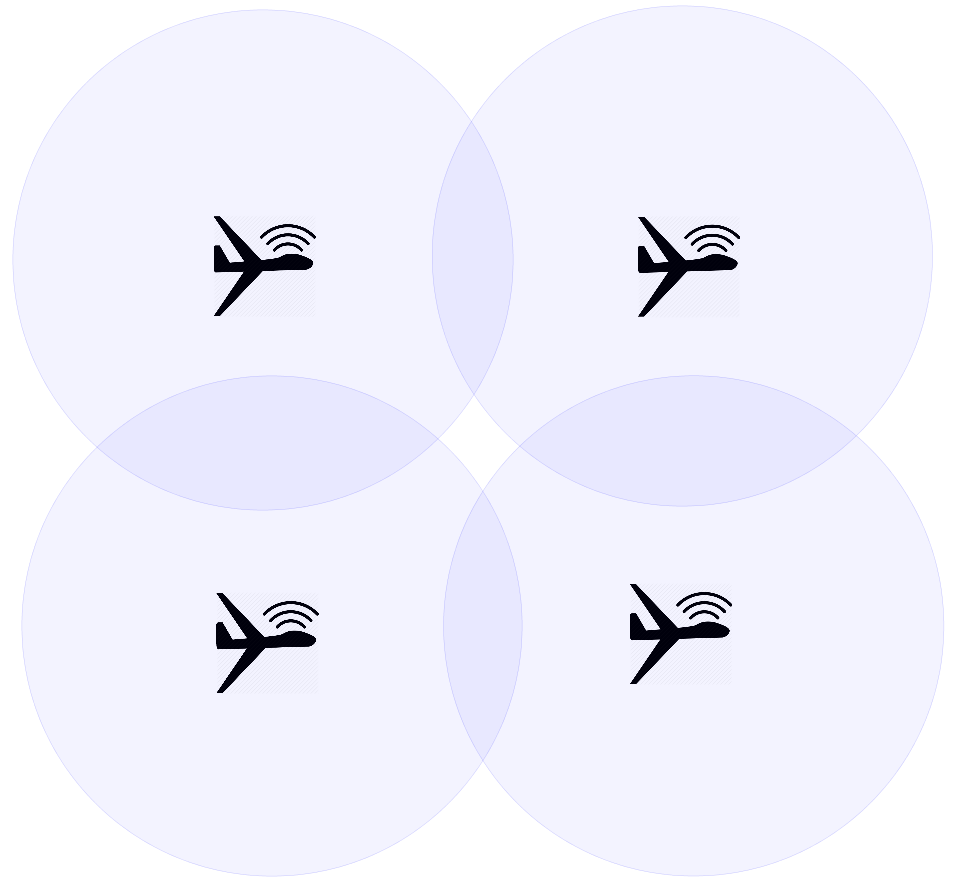
\includegraphics[width=0.35\textwidth]{Figures/conn1.png}} 
      \subfloat[Connected network.]{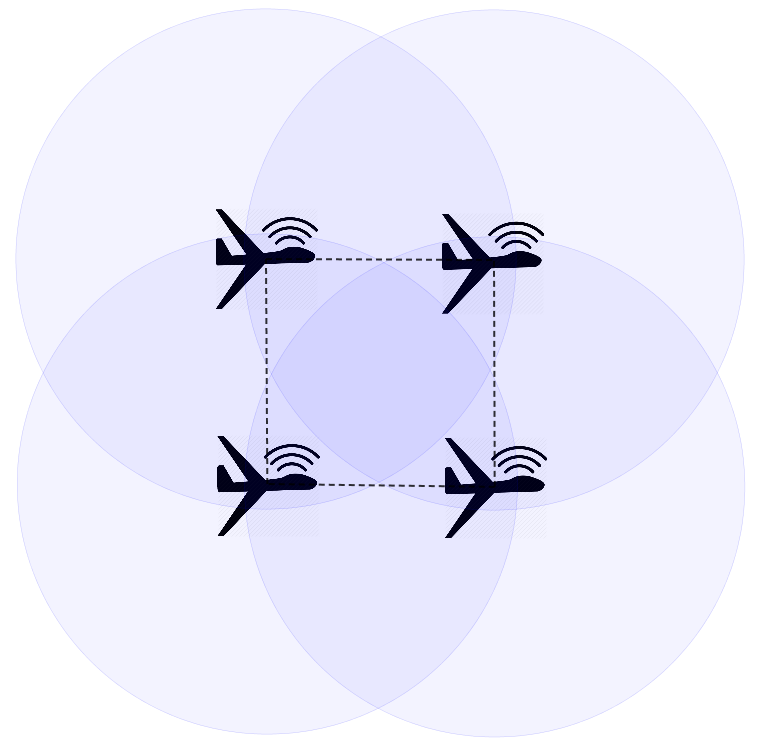
\includegraphics[width=0.35\textwidth]{Figures/conn2.png}}   \\ \centering
       \caption{Communication topology in a collaborative UAV network.}
    \label{fig:communicationLink}
\end{figure}


Threats are represented by circles, defined by their center position (physical radar position) and detection range. In order to respond to threats, the UAVs must be able to detect them during flight. Given that the threat range is normally larger than the detection range of an UAV, the detection of these radars is often given by passive receivers, which can be used to detect radar emissions over considerable distances \cite{gross_2007}. In this regard, we consider that the UAVs are equipped with Radar Warning Receivers (RWRs), which are able to detect the emissions from the threats. 

In this work, the UAV objective is to fly from the start position to a common goal position using a collaborative approach to detect and avoid threats, using an active stealth policy. To reproduce the scenario, we propose a simulation model over a time interval $t=[t_0..t_{max}]$. Since we do not consider lethal threats such as FCRs, all UAVs will achieve the goal. If all UAVs reach the goal before $t_{max}$, the mission is considered accomplished. A specific scenario consisting of UAVs performing collaborative tasks in hostile environments is presented in Figure \ref{fig:scenario}. In this figure, the threats are represented by the red circles.

\begin{figure}[h!]
    \centering
    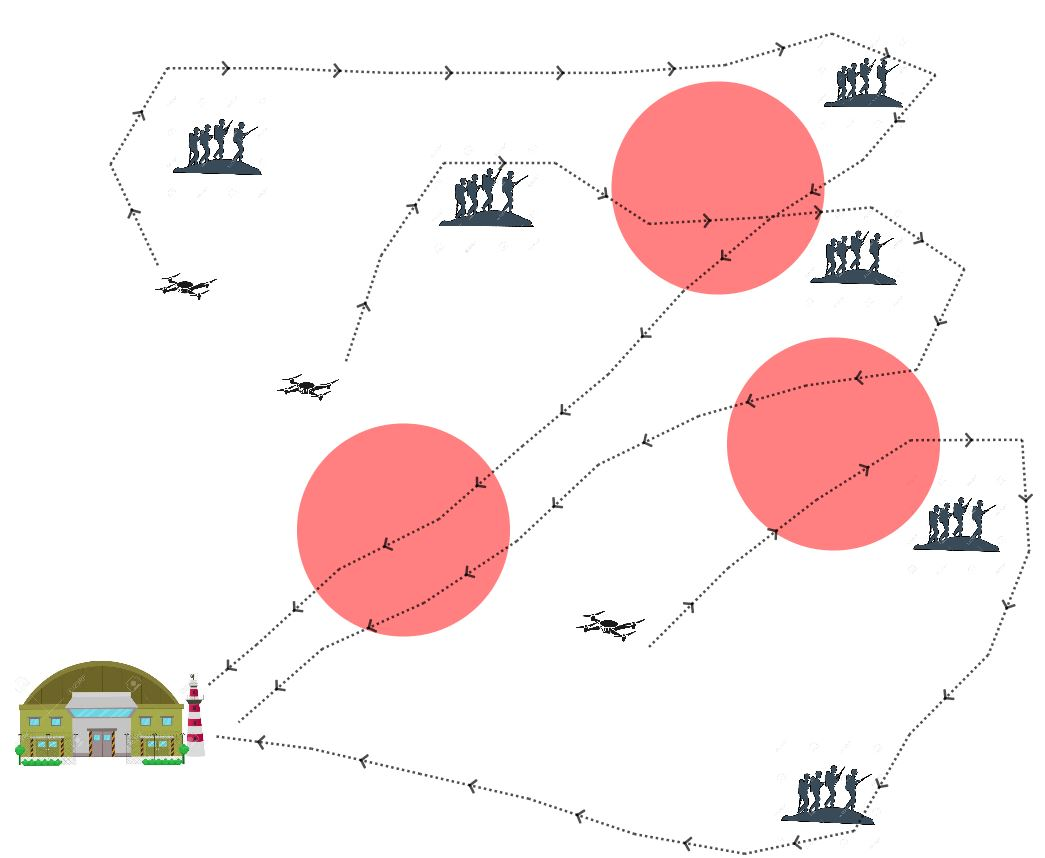
\includegraphics[width=0.6\textwidth]{Figures/scenario.png}
    \caption{An instance of the proposed scenario.}
    \label{fig:scenario}
\end{figure}

Notice that, for this scenario, the UAV network is fragmented into two local networks, since these networks are further from each other than the communication range of the UAVs. Moreover, these local networks are totally independent. There will only be collaboration between these two networks if at least one UAV of each of the networks communicates, thus unifying the networks. The remainder of this chapter details the proposed model. 

\section{Threat identification}

Due to the fact that our model considers that the detection of threats by the UAVs is passive, it is important to differentiate the concepts of detection range and detectability range. According to \cite{adamy2004}, a radar's detection range is the range at which it can detect a target, while the detectability range is the range at which its signal can be received and detected by a receiver.
 
This work is not focused on modelling electronic aspects of signals for the detection of a threat by the RWR or the detection of an UAV by a surveillance radar, but in modelling an stealth approach in collaborative UAV networks. Thus, the radar modelling is simplified as a range for detection. A threat is considered detected by an UAV if its range overlaps the RWR range, and an UAV is considered detected by a threat if the UAV is inside its detection range, as shown in Figure \ref{fig:rwr}. It is possible to notice that, in this case, the UAV is detecting the threat but the threat does not know about the presence of the UAV, because this is not in its detection range. 

\begin{figure}[h!]
\centering
\includegraphics[width=0.40\textwidth]{Figures/rwr.png}
\caption{Threat identification with RWR.}
\label{fig:rwr}
\end{figure}

Beyond the knowledge about the presence of a radar, when the RWR detects a threat, the detection range of this threat must be estimated so that other UAVs can avoid this region. The first step to estimate the threat region consists in calculating the electronic position of the threat. According to \cite{exercito_2009}, the electronic positions are commonly estimated by two different approaches: Direction Find (DF) and Time of Arrival (TOA). The DF is the technique used in most electronic localization systems due to low cost and simplicity. It analyses the direction of the emitted electromagnetic waves and can be implemented by two distinct processes:

\begin{itemize}
    \item \textbf{Horizontal localization:} The electronic position of the target is estimated by receivers and special systems of antennas that allow to establish the direction of the emissions. If measurements are made from properly spaced points, the intersection of these directions will indicate a probable area of the sender's location. This technique can be implemented using two approaches: using several UAVs, that detects a threat simultaneously or with a single equipment, performing azimuth measurements in successive positions. Figure \ref{fig:horizontalLoc1} shows an example of horizontal localization using different UAVs, while Figure \ref{fig:horizontalLoc2} presents an example of horizontal localization using a single UAV in different moments. 
        
    \begin{figure}[h!]
      \centering
      \subfloat[Using different UAVs.]{\includegraphics[width=0.4\textwidth]{Figures/eletronicLocalization1.png}\label{fig:horizontalLoc1}}
      \subfloat[Using a single UAV.]{\includegraphics[width=0.4\textwidth]{Figures/eletronicLocalization2.png}\label{fig:horizontalLoc2}}
      \caption{Horizontal localization.}      
    \end{figure}
    
    \item \textbf{Vertical localization:} The electronic position of the target is estimated by systems that use only one station to provide the coordinates of the opposing sender. In this technique, the direction of arrival and the height of the ionosphere are used to estimate the origin of the signal. This technique is only efficient for electromagnetic signals in the frequency range of HF, which suffer refraction in the ionospheric layer.
\end{itemize}

On the other hand, TOA consists in verifying the time between the electromagnetic pulses. This technique is more complex than DF, however it is more precise w.r.t. threat position estimation. If the exact moment at which the signal is emitted is known, for instance using an RWR, it is possible to estimate the threat's position. When the receptor detects the signal, a circumference is calculated with the distance between the receiver and the target. By intersecting two or more circles, it is possible to determine the location of the target \cite{exercito_2009}. In the same way that occur with Horizontal Location, this approach can be used by more than one UAV, as shown in Figure \ref{fig:DFOA1}, or using a single UAV in different moments, as shown in Figure \ref{fig:DFOA2}.

   \begin{figure}[h!]
      \centering
      \subfloat[Using different UAVs.]{\includegraphics[width=0.49\textwidth]{Figures/eletronicLocalization4.png}\label{fig:DFOA1}}
      \subfloat[Using a single UAV.]{\includegraphics[width=0.49\textwidth]{Figures/eletronicLocalization3.png}\label{fig:DFOA2}}
      \caption{Difference time of Arrival.}      
    \end{figure}

The exact moment at which the signal is emitted is sometimes unknown. Even in this case, it is also possible to estimate the radar location by Time of Difference Arrival (TDOA), which  is a technique based on the premise that any transmitted signal will arrive at different times in the receiver on the ground. From some mathematical analysis, it is possible to draw parabolas that will coincide at a certain point to determine the coordinates of the emitting target \cite{exercito_2009}.

This work does not intend to address the procedure of electronic localization and the error from position estimation. When an UAV detects the presence of a threat, it is assumed that the threat position is precisely known and its detection range can be calculated by:

\begin{equation}
R' = \sqrt{(P_x - P'_x)^2 + (P_x - P'_y)^2} - R,
\label{eq:threatRange}
\end{equation}

where $R$ is the RWR range of the UAV, $P'$ is the threat's position and $R'$ is its detection range.

Once we are considering that all the UAVs are equipped with an RWR, our model can uses a communication model based on intrusion detection described in \cite{farhan_2010}. Intrusion detection communication models can be classified into three groups:

\begin{itemize}
    \item \textbf{Standalone:} every node makes the detection without collaborating with others.
    \item \textbf{Distributed and Cooperative:} each node detects intruders as in the standalone approach, but communicate with other mobile nodes to exchange attack data for supporting global decisions making and agreeing on responses
    \item \textbf{Hierarchical:} the detection procedure is generally divided into small groups, such as clusters, and zones where some mobile nodes have more responsibility than others in the same group.

\end{itemize}

The Distributed and Cooperative is the model which most applies to our scenario. In our context the intruders are the threats. Based on this, every time an UAV detects a threat, a Depth-First Search procedure is applied in order to identify the UAVs that are connected to this node \cite{tarjan_1972}. These UAVs have their list of known threats updated and their path recalculated to avoid the new threat.

For stealthiness purposes, the UAVs that detect a threat cannot continue sharing information while in a critical area, otherwise the content of the communication could be heard by an passive radar. Thus, a safety distance must be added to the estimated threat range. At this moment, we are considering this new threat range as the union of the communication range of the UAV and the estimated detection range of the threat. We named this as \emph{Virtual Range} of the threat.

This approach is justified because we are assuming that the surveillance radars are in strategic locations, where it is essential to know the presence of enemy aircraft. Therefore, the probability of the presence of passive radars in this region is high, since some aircraft has some features that makes its detection harder by using surveillance radars. The UAVs may have different types of equipment, but for the collaborative approach adopted in this work, we consider that it is equipped with RWR and a communication radar. As the RWR is a signal receiver, it is not necessary to turn it off. Thus, the UAV will only turn the communication radar on again when the RWR does not detect the presence of any threat.  

\section{UAVs displacement model}

Given that each UAV state is its position $p_i\in\mathbb{R}^m$,  and \mbox{$p=\left[p_1^T\ldots p_N^T\right]^T\in\mathbb{R}^{N \times m}$} is the state vector of the multi-UAV system. Assume that each UAV can be modeled as a single integrator system and its velocity can be directly controlled, namely:

\begin{equation}
\dot{p}_i = u_i,
\label{eq:singleintegrator}
\end{equation}

where $u_i\in \mathbb{R}^m$ is a control input.

Consider a scenario where the UAVs must perform a mission using a collaboratively approach. Several factors must be taken into account in order to do so without compromising the success of the mission. For instance, the UAVs must avoid the enemy radars. Moreover, depending on the kind of mission, they must improve or decrease the coverage area, or improve the level of robustness to failures of the overall network. Based on this, the UAVs displacement can be modelled as a combination of control laws and adaptive gains. The combined control law for supporting the movement of UAV $u_i$  is then defined as:

\begin{equation}
u_i=\tau u_i^p + \sigma u_i^c + \rho u_i^r + \phi u_i^v
\label{eq:integratedcontroller}
\end{equation}

where: 

\begin{itemize}
    \item $u_i^p$ is the control law responsible for the the path planning and enemy radars avoidance.
    \item $u_i^c$ is the generalized connectivity maintenance control law;    
    \item $u_i^v$ is the control law responsible for improving the coverage area;
    \item $u_i^q$ is the control law responsible for improving the robustness to failures;    
    \item $\tau$, $\sigma$, $\rho$ and $\phi$ are the adaptive gains of the control laws.
\end{itemize} 

This work extends the combined control law model described in Ghedini \cite{ghedini_2017}, by increasing the path planning control law $u_i^p$. This displacement model is based on differential equations. Notice that if an adaptive gain is zero, its corresponding control law is inactive, i.e, the UAV does not need to change its position regarding the respective control law. The control laws are addressed as follows. For instance, considering a scenario in which the gain settings are $\tau=1$, $\sigma=75$, $\phi=1$ and $\rho=0$. In this case, each UAV must move trough the planned path to increase both its sensing area, without increasing its robustness to failure, while keeping the global network connectivity and avoiding collision with other UAVs.

There are different displacement models in literature, such as the described in He and Dai \cite{he_2013}. In this model, the movements of the UAVs are determined by optimization of factors under movement constraints with genetic algorithm.  A problem when using optimization models based on genetic algorithms is the computational cost for the model to converge. Considering that our scenario is very dynamic, where the drones need to recalculate their flight routes several times due to the detection of enemy radars, a model based on differential equations, such as described in Ghedini \cite{ghedini_2017}, ends up being more advantageous.

\subsection{Path trajectory control law $u_i^p$}
Flying towards the target the UAVs perform dynamic detection of the threats. Once a threat is detected, it is necessary to replan a trajectory to avoid this region. Each UAV autonomously calculates its own path. However, depending on the application, the UAVs should fly using different approaches. Thus, a procedure to define the goal position of UAVs using local information is necessary. This section presents the control law responsible for driving an UAV $u$ to follow a path that avoids the threat regions.

\subsubsection{Flight path approaches}

There are several flight formations for conventional airplanes, however some of them are not applicable to UAV scenarios because in the context of unmanned aircraft, there is no concept of a pilot's vision range. As aforementioned, this works consider that the sensing mechanisms usually present in UAVs are the radar for communication and the RWR. Therefore, the flight formation can only consider these.

Different kind of missions may require different formations. We consider two kinds: a structured flight formation that minimizes the exposure of UAVs to threats and a unstructured flight approach that add mechanisms that allows coverage control and robustness to failure improvement. We describe these approaches in what follows.

\subsubsection{Structured flight approach}

According to \cite{giulietti_2000}, in a typical flight formation there are the roles of leader and wingmen. In this context, the wingmen follow the trajectory of the leader, taking the other aircrafts as a reference to keep its own position in the formation. The leader's responsibility is to define the trajectory to the goal. In a rigid flying formation, inter-aircraft distances must be kept constant. 
 
In hostile environments, where the UAVs do not have information about the threat location, exposure should be reduced. In this sense, there is a flight formation, described in \cite{borges_2017}, named trail, that is used to air-to-ground attack on dangerous environments. Figure \ref{fig:trailFormation1} presents an example of the trail formation. The numbers above the UAVs correspond to their formation ranking ($id$). The UAV with $id$ $1$ is the leader of the connected component and responsible for calculating the trajectory to the goal, while the others are the wingmen, which always calculate the trajectory to the successor, i.e., the UAV that has $id = a -1$, where $a$ is the current UAV $i$. The problem with such formation is that the UAVs are not supported by any other UAV in formation, consequently, if one of them fails or is hit by an enemy, the UAV communication network can easily become disconnected.
  
\begin{figure}[ht]
\centering
\includegraphics[width=.45\textwidth]{Figures/trailFormation1.png}
\caption{Trail formation for UAVs.}
\label{fig:trailFormation1}
\end{figure}

For generating this formation, the UAV that is chosen to be the leader of a connected component of the network is the UAV that has the shortest path to the goal. The other UAVs' ranking are generated based on the length of their path to the leader: the closer an UAV is to the leader, the lower is its ranking position. The formation ranking, however, cannot be static because the connection between two UAVs may be lost. There are two reasons for connectivity loss between UAVs in the proposed scenario: the first one occurs because the distance between the UAVs are greater than its communication range. The second one is due to the fact that an UAV can turn off its communication radar. Thus, it is essential for the communication that these situations are detected so that UAVs take actions to reestablish the formation as quick as possible \cite{giulietti_2000}. 

Another possible scenario where it is necessary to update the flight formation is when there are two connected components that are close enough to be merged. For updating  a flight formation, the number of connected UAVs within a formation ranking $1$ is verified. If there are more than one, the leader will be the UAV with formation ranking $1$ that has the shortest path to the goal. We choose as leader the UAV with the shortest path to goal instead of the UAV that is closest to the goal because, since the scenario contains threats that must be avoided and it is not possible to ensure that the UAV that is closest to goal will reach the goal earlier. Figure \ref{fig:trailFormation0} presents an example of scenario where two flight formations are merged. There are two UAVs with $id=1$. The one that is below is closest to goal, however, due to the presence of threats, its path to the goal is longer than the path of the other UAV with $id=1$.

\begin{figure}[hbt!]
      \centering            
      \subfloat[Before merge formation.]{\includegraphics[width=0.35\textwidth]{Figures/trailFormation0.png}}      
      \subfloat[After merge formation.]{\includegraphics[width=0.35\textwidth]{Figures/trailFormation0_1.png}}
      \caption{Leader selection during a formation merging procedure.}     
      \label{fig:trailFormation0}
\end{figure}


The other UAVs rank indexes are updated based on their distance to the new leader, as previously described. Figure  \ref{fig:trailFaulExample1} illustrates a connectivity loss, while the resulting ranking reconfiguration is presented in \ref{fig:trailFaulExample2}. On the other hand, Figure \ref{fig:MergeFormations} illustrates how two flight formations are merged.

\begin{figure}[h!]
      \centering            
      \subfloat[Before fragmentation.]{\includegraphics[width=0.35\textwidth]{Figures/trailFormation2.png}\label{fig:trailFaulExample1}}      
      \subfloat[After fragmentation.]{\includegraphics[width=0.35\textwidth]{Figures/trailFormation3.png}\label{fig:trailFaulExample2}}            
      \caption{Connection fault example.}     
      \label{fig:trailFaulExample}
\end{figure}

\begin{figure}[h!]
      \centering            
      \subfloat[Start scenario.]{\includegraphics[width=0.35\textwidth]{Figures/trailMerge1.png}}      
      \subfloat[Update formation Id.]{\includegraphics[width=0.35\textwidth]{Figures/trailMerge2.png}}     \\
      \subfloat[Start move UAVs.]{\includegraphics[width=0.35\textwidth]{Figures/trailMerge3.png}}      
      \subfloat[Trail formation established.]{\includegraphics[width=0.35\textwidth]{Figures/trailMerge4.png}\label{fig:trailMerge4}}      
      \caption{Merge two formations in trail.}     
      \label{fig:MergeFormations}
\end{figure}

\subsubsection{Unstructured flight approach}

Using a structured flight approach, such as the trail, does not make possible to change the UAVs position for different tasks, for instance for coverage area improvement, as the formation can be undone. The unstructured flight approach we are using consider that each UAV will calculate its own path to the goal. Therefore, there is no leadership between UAVs. Figure \ref{fig:unstructuredFlightFormation} illustrates a scenario in which the UAVs are flying using an unstructured flight formation. 

\begin{figure}[ht]
\centering
\includegraphics[width=.45\textwidth]{Figures/unstructuredFormation.png}
\caption{Example of unstructured flight formation.}
\label{fig:unstructuredFlightFormation}
\end{figure}

There are different paths from a starting point to the goal using a non-deterministic algorithm for path planning such as RRT. In order to have a connected network, it is essential that the trajectories calculated by UAVs that are connected do not differ too much. In this context, it is possible to apply some curve similarity metric for evaluating how close two paths are in order to match them. There are several curve similarities metrics, two of them are the  Discrete Fr{\'e}chet Distance (DFD) and the Modified Hausdorff Distance (MHD).

The DFD is a variation of the Fr{\'e}chet distance for using with polygons. This metric searches for all coupling possibilities between the polygon end points. Given two curves $f:[a, b] \rightarrow V $ and $g:[a_r, b_r] \rightarrow V$, the distance $D$ can be calculated as follows \cite{eiter_1994}: 

\begin{equation}
D = \delta(f,g) = \inf_{\alpha, \beta \in [0,1]} max[f(\alpha(t)), g(\beta(t))]
\end{equation}

The MHD is a variation of the Hausdorff distance. For applying this distance to two curves $f:[a, b] \rightarrow V $ and $g:[a_r, b_r] \rightarrow V$ , it is necessary to build a distance vector ($v$) for $f$ and a distance vector ($vr$) for $g$. Then, given a point $x \in f$, each position of $v$ is defined as the minimum distance from $x$ to the points belonging to $g$. In addition, given a point $y \in g$, each position of $vr$ is defined as the minimum distance from $y$ to the points belonging to $f$. The MHD is the maximum value between the average of $v$ and the average of $vr$. The closer the DFD or the MHD between two paths are to 0, the closer the paths are.  Our model uses the DFD for evaluating the path similarity \cite{dubuisson_1994}.

We propose a matching procedure that consists in defining a reference path and, based on it, try to match the path of others UAVs to it. The first step to perform this procedure consists in finding the reference path. In this direction, the UAVs are grouped based on the similarity between their paths. If the DFD between two UAVs paths is less than a threshold, the UAVs are considered to belong to the same group. The reference path will be the path closest to the goal of the UAV that is inside the group with the large amount of UAVs. If there are two or more groups with the same amount of UAVs, the reference path will be the best candidate of those groups whose path is closest to the goal. The procedure of matching is iterative, as illustrated by the activity diagram in Figure \ref{fig:unstructuredFormationDiagram}. Figure \ref{fig:refPathMatching} presents the result of an application of the matching procedure. The current position of the UAVs are represented by the blue points, while the goal of the mission is represented by a red point. The black circles are the threats, with the continuous line constituting the detection range of the enemies radars, while the broken line represents the virtual range of the threat. Notice that all the paths become close to each other and, as a consequence, the likelihood of a network disconnection decreases, which is desirable for cooperative tasks.

\begin{figure}[hbt!]
\centering
  \includegraphics[width= 0.5\linewidth]{Figures/unstructuredFormation1.png}
  \caption{Activity diagram of the reference path matching procedure.} \label{fig:unstructuredFormationDiagram}
\end{figure}

\begin{figure}[hbt!]
      \centering            
      \subfloat[Before executing the path matching.]{\includegraphics[width=0.45\textwidth]{Figures/unstructuredFormation2.png}\label{fig:unstructured}}      
      \subfloat[After executing the path matching.]{\includegraphics[width=0.45\textwidth]{Figures/unstructuredFormation3.png}\label{fig:unstructured2}}
      \caption{Reference path matching example.}     
      \label{fig:refPathMatching}
\end{figure}

The procedure used for computing the flight path planning in both flight formation approaches is addressed as follows. 

\subsubsection{Flight path planning}

Since each UAV knows the position that it must reach to accomplish the mission, each of them calculates its own path to the goal. There are two situations for path planning: when an UAV is inside a threat region (communication radar is turned off), and when a UAV is outside a threat region. With regard to the algorithm for path planning, the difference between these scenarios depends on the definition of the goal position. By default, the goal position of the UAVs is influenced by the approach they are flying. In the case of the structured formation, the wingmen follow the leaders. On the other hand, by using the unstructured approach there is no leadership. All the UAVs calculate the paths directly to the goal of the mission. The case when an UAV is exposed to a threat will be addressed later.

Considering that RRT is a widely used technique for path planing with obstacle avoidance for UAVs, we use this algorithm as reference for computing the path planning. The Algorithm \ref{alg:rrt} shows how RRT computes the path planning from current position to a goal position. 

\begin{algorithm}
\caption{RRR algorithm - Compute path}\label{alg:rrt}
\begin{algorithmic}[1]
\Procedure{ComputePath}{$p_{current}$, $p_{goal}$, $p_{obstacles}$, $n_{edges}$, $e_{length}$, $n_{max}$} 
\State $G\gets Graph(p_{current})$ \Comment{Current position is the first vertex of the graph.}
\State $i\gets 1$
\State $k\gets 1$
\While{$k\leq=n_{edges} \And i\leq=n_{max}$}
\State $q_{rand}\gets CreateRandomPoint()$
\State $q_{near}\gets NearestVertex(q_{rand}, G)$
\State $q_{new}\gets TruncateEdge(q_{near}, q_{rand}, e_{length})$
\If{$\neg Intercept(q_{new}, p_{obstacles})$}
\State $G.addVertex(q_{new})$
\State $G.addEdge(q_{near}, q_{new})$
\State $k\gets k+1$
\EndIf
\State $i\gets i+1$
\EndWhile\label{euclidendwhile}
\State $p_{near}\gets ClosestVertexToGoal(G, p_{goal})$ \Comment{Get vertex that is closer to the goal}
\State $path\gets G.ShortestPath(1, p_{near})$
\State \textbf{return} $path$
\EndProcedure
\end{algorithmic}
\end{algorithm}

A limitation of RRT is not consider the movement constraints of the UAVs. Thus, we use an adaptation of this method for avoiding invalid movements based on angle validation. RRT has as inputs a start point $p_0$, the number of branches $n_e$ and a distance $d$. The initial tree contains only $p_0$. Then, a random position in the scenario is generated and the nearest node $k_n$ to this position in the tree is searched. Once the node is identified, a line $l$ that passes along these two nodes is generated. Next, a line segment of length $d$, starting from $k_n$, is extracted from $l$. If the line segment does not pass thought any forbidden region (zone around a threat, in our case), this branch is added to the tree. This process is repeated until the number of branches is equal to $n_e$ or when the number of iterations is greater than a threshold. Taking into account that there is no guarantee that RRT will provide a feasible path to the goal, the UAVs will always move towards the nearest position of the goal $p_f$, considering the tree generated by RRT. The shortest path between the start position and $p_f$ is computed using the Dijkstra algorithm \cite{dijkstra_1959}.  The resulting tree is highlighted in Figure \ref{fig:rrt1}. 

\begin{figure}[hbt!]
\centering
\includegraphics[width=.7\textwidth]{Figures/rrt1.png}
\caption{Path generated by RRT.}
\label{fig:rrt1}
\end{figure}

\subsubsection{Angle validation}

Since it is more important for the present model to evaluate the behavior of the UAV network according to a stealth policy and a combined control law and not modeling a large set of handling dynamical restrictions, such as yaw and pitch angles, described in \cite{he_2013}, we adopt a single handling constraint, which is the angle variation between movements.

Every time a UAV moves from position $P_1$ to a new position $P_2$ the angle between these points is calculated. The equation for calculating the angle $\epsilon$ between  $P_1$ and $P_2$ is described by:

\begin{equation}
    \epsilon = atan2(y,x), 
\end{equation}

where $y$ is the difference between the y-axes value of $P_1$ and $P_2$ and $x$ is the is the difference between the x-axes value of $P_1$ and $P_2$. The function $atan2(y,x)$ is the function $tan^{-1}(\frac{y}{x})$, limiting the resulting angle in the range of $[-pi, pi]$.

For avoiding invalid movements, an UAV movement will only be considered valid if the angle generated by the new and current positions is in a specific range, as illustrated in Figure \ref{fig:flightAngle}. In this figure, the UAV flights from position $P_{i-1}$ to $P_i$. The angle between $P_i$ and the next movement must not exceed the max angle variation $\theta$, otherwise it will be considered an invalid movement.

\begin{figure}[hbt!]
\centering
\includegraphics[width=.6\textwidth]{Figures/angleVariation.png}
\caption{Angle validation of UAV movement}
\label{fig:flightAngle}
\end{figure}

In terms of implementation, a solution to use this approach is to adapt the RRT algorithm to only generate branches of the tree if the angle generated by the new intermediate goal point and the nearest node in the tree is in a specific range. Figure \ref{fig:pathWithAngleRestriction} presents the resulting branches (black lines) and the path generated by the execution of RRT (green lines) with and without angle restrictions for different values of $\epsilon$. The red circles represents the threats.

\begin{figure}[hbt!]
      \centering            
      \subfloat[Resulting path with $\epsilon$ = 90$\degree$. ]{\includegraphics[width=0.45\textwidth]{Figures/rrt90.PNG}}      
      \subfloat[Resulting path with $\epsilon$ = 60$\degree$.]{\includegraphics[width=0.45\textwidth]{Figures/rrt60.PNG}}  \\ \centering
      \subfloat[Resulting path with $\epsilon$ = 45$\degree$.]{\includegraphics[width=0.45\textwidth]{Figures/rrt45.PNG}} \caption{Generated path with angle validation.}
      \label{fig:pathWithAngleRestriction}     
\end{figure}

\subsubsection{Path reduction}

Since the output of RRT is a set of consecutive lines, it is possible to optimize the path to reduce its length. This procedure consists in attempting to trace the longest lines as possible between path vertexes. Figure \ref{fig:pathReduce} illustrates an example of the path reduction procedure, notice that it significantly changes the original path provided by RRT. It is important to note that the new lines are restricted to the valid angle range condition aforementioned.

\begin{figure}[hbt!]
\centering
\includegraphics[width=0.9\textwidth]{Figures/RRT_Reduce.png}
\caption{Path reduction example.}
\label{fig:pathReduce}
\end{figure}

The result of the procedure to reduce paths provides a path where the vertices are located at varying distances. The UAV needs to move by following the path according to a reference speed, then it is necessary to know the position that the UAV would be at the moment $t$ within the previously computed path. Thus, by using interpolations, new equidistant vertexes are generated \cite{davis_1975}. The distance between them is proportional to the speed of the UAV.

\subsubsection{Path smoothing}

RRT provides, as output, a linear piecewise representation of the trajectory. Thus, it may be necessary to apply a path smoothing method for generating feasible trajectories, as highlighted in \cite{borges_2016}. The smoothing procedure considered here is based on an algorithm proposed to perform horizontal segmentation of highways \cite{coelho_2015}. The first step of this algorithm consists of identifying the instant that the angular coefficient varies, as shown in Figure \ref{fig:pathSmoothing1}. Given these moments, a set of neighbours are selected, as presented in Figure \ref{fig:pathSmoothing2}. 

\begin{figure}[h!]
      \centering            
      \subfloat[Detection of angular coefficient variation.] {\includegraphics[height=0.35\textwidth,width=0.45\textwidth]{Figures/PathSmoothing1.eps}\label{fig:pathSmoothing1}}      
      \subfloat[Derfining in neighbourhood.]{\includegraphics[height=0.35\textwidth,width=0.45\textwidth]{Figures/PathSmoothing2.eps}\label{fig:pathSmoothing2}}  \\ \centering
      \caption{Angular coefficient variation detection.}
\end{figure}

Taking into account the set of computed points, a circle is fit \cite{coope_1993}, resulting in the radius and center coordinates of the circle that best adjust to the set of points, as shown in Figure  \ref{fig:pathSmoothing3}. Computed the circle fitting, it is necessary to select the points in the circles that correspond to the points of the neighborhood used for fitting, as presented in Figure \ref{fig:pathSmoothing4}. 

\begin{figure}[h!]
      \centering            
      \subfloat[Circle fitting.]{\includegraphics[height=0.35\textwidth,width=0.45\textwidth]{Figures/PathSmoothing3.eps}\label{fig:pathSmoothing3}}      
      \subfloat[Select points in circles.] {\includegraphics[height=0.35\textwidth,width=0.45\textwidth]{Figures/PathSmoothing4.eps}\label{fig:pathSmoothing4}}  \\ \centering
      \caption{Circle fitting procedure}
\end{figure}

The next step consists in replacing the neighbourhood points by the points in the generated circles, as shown in Figure \ref{fig:pathSmoothing5}. Finally, a moving average procedure is executed in order to match lines and curve regions \cite{azami_2012}. Figure \ref{fig:pathSmoothing6} illustrates the path after the execution of successive moving average procedures.

\begin{figure}[h!]
      \centering            
      \subfloat[Replacing points in neighbourhood] {\includegraphics[height=0.35\textwidth,width=0.45\textwidth]{Figures/PathSmoothing5.eps}\label{fig:pathSmoothing5}}      
      \subfloat[Path after moving average procedure.] {\includegraphics[height=0.35\textwidth,width=0.45\textwidth]{Figures/PathSmoothing6.eps}\label{fig:pathSmoothing6}}  \\ \centering
      \caption{Path after path smoothing procedure.}
\end{figure}

\subsubsection{Computing the goal for an UAV in a threat region}

The stealth policy of turning off the communication radar adopted here consider that the UAV that enters a threat region cannot communicate with other UAVs. Moreover, the UAV must trace a path to leave the area of the threat. In this sense, there are two approaches for computing the goal, which is used as reference for path planning, to leave the threat region: the first one implies leaving the threat region quickly, while the other approach consists in computing the goal position in a region that the other UAVs of the formation will possibly pass through, thus improving the chance for the UAV that turned off the radar to regroup with the others.

The procedure for computing a goal for the UAV in a threat region assumes that each UAV knows its own position $p_i$ and its neighbor positions $p_{\mathcal{N}_i}=\{p_j,\forall j\in\mathcal{G}: i,j \in \mathcal{E}\left(\mathcal{G}\right)\}$.

The first step consists in generating candidate points that allows the UAV to leave the threat region. An UAV has two candidate points $P_i'$ and $P_i''$, one at each direction. These points are obtained from the equation of the line $L_{Proj}$ that passes through the last position of the UAV $P_{i-1}$ and its current position $P_i$. The candidate points  $P_i'$ and $P_i''$ are the first points that are outside the threat, considering the line $L_{Perp}$ which is perpendicular to $L_{Proj}$ and pass through the center of the threat. Figure \ref{fig:LeaveThreat1} illustrates the procedure to compute the candidate points.

\begin{figure}[hbt!]
\centering
\includegraphics[width=0.65\textwidth]{Figures/leaveThreat1.png}
\caption{Candidate points for computing path planning to leave threat region}
\label{fig:LeaveThreat1}
\end{figure}

The next candidate point $P_i'''$ results from the estimation of future positions of connected UAVs. While in the trail formation, we have the leader and the wingmen, in the unstructured approach there is no leadership. Therefore, the procedure for estimating the future position of UAVs is different for these flight formation approaches and are described as follows.

\subsubsection{Trail formation}

The procedure for estimating the future position of the UAVs flying using the trail formation is straightforward. The UAV that is exposed to a threat will compute the path to the goal, considering that is in the last position of its successor into the flight formation. 

RRT it is not a stochastic algorithm, thus it is not ensured that the path of the successor and the estimated path will coincide. On the other hand, because of threat avoidance, the angle validation and the path reduction procedure, the chance of these paths coinciding is high. The estimated path position $P_i'''$ is the point in the computed path that is closest to the previously computed candidates $P_i'$ and $P_i''$, as shown in Figure \ref{fig:LeaveThreat2}.

\begin{figure}[h!]
\centering
\includegraphics[width=0.8\textwidth]{Figures/leaveThreat2.png}
\caption{Candidate points for computing path planning to regroup with the other UAVs.}
\label{fig:LeaveThreat2}
\end{figure}

\subsubsection{Unstructured flight approach}

Considering that there is no leadership in the unstructured flight approach, it is not possible to estimate the future position of UAVs by computing the path of an UAV's successor in formation. Thus, it is necessary to consider the paths of all UAVs that are connected with the UAV that turned off the communication radar

The UAV that is exposed to a threat will compute the paths to the goal of all its neighbours. Thus, the UAVs are clustered based on the DFD between their computed paths. Whether the DFD between two UAVs' paths is lower than a threshold, these are considered belonging the same group. A large amount of UAVs in the same group indicates that the most part of UAVs tends to fly using a nearby path. Therefore, the chance of estimating correctly the future position of the UAVs increases. In this direction, considering that maybe exist more than a group with the same amount of UAVs, for each path in the groups with the most amount of UAVs, the points $P_i^j$ that are close to the previously computed candidates $P_i'$ and $P_i''$ are selected. 

The next step consists in compute the average point $P_i^javg$ for each previously computed points $P_i^j$. Then, the estimated path position $P_i'''$ is the point $P_i^javg$ which results int the shortest path length between current UAV position and $P_i^javg$. By using this approach, we improve the chance of the UAV reconnect with other uavs due to the fact that we drive the UAV to a position in which the most UAVs of the network will probably pass near.

\subsubsection{Selection of the best candidate point}

Once the candidate points $P_i'$, $P_i''$ and $P_i'''$ were computed, it is necessary to establish the criterion for which candidate point should be the goal of the UAV. If $P_i'''$ exists\footnote{$P_i'''$ can only be computed in the case that the UAV is connected to another UAV.}, this point is outside a threat region and the path length from the current UAV position to $P_i'''$ does not exceed a maximum length threshold $L_{max}$, this candidate point is selected to be the goal. Otherwise, the choice is between $P_i'$ and $P_i''$. Thus, the goal is the candidate that is outside a threat region, whose path length between the current UAV position and these two candidate points is smaller. 

Notice that if there is no candidate point that meets the constraints, for instance in the case of all candidates inside threat regions, the goal that supports the path planning to leave the threat region will be the goal of the mission. However, in order to avoid flying over the physical position of the radar (center of threat region), the path planning consider the threat range to be lower than it actually is, making the UAV fly across the edges of the detection range. 

\subsubsection{Displacement model}

The objective of this control law is to drive the UAV $u$ to follow a path that avoids the threat regions, given a path $Path\gamma(u)$ of the UAV $u$, located at the position $p_i$ at a moment $t$. By using interpolation, it is possible to estimate the position $x_\gamma^i$ in which the UAV should be at a moment $t+1$, following $Path\gamma(u)$. Notice that the distance from positions $p_i$ and $x_\gamma^i$ is  parameterized and impacts the speed of the UAV in our model. Thus, the control law that drives the UAV $u$ to follow the path planning is defined by:

\begin{equation}
u_i^p = \tfrac{x_\gamma^i - p_i}{\left\| x_\gamma^i - p_i \right\|}\beta\left(t\right),
\label{eq:controllawPathPlanning}
\end{equation}
where $\beta\left(t\right)\in\mathbb{R}$ is the linear velocity of the UAVs.

Due to the performance purposes the path planning algorithm does not have to be executed at each iteration $t$. For instance, considering a scenario where the UAV $u$ does not shut down its communication radar and that the straight segment that passes through $p_i$ and $x_\gamma^i$ does not intercept any threat regions, and the generated angle between $p_i$ and $x_\gamma^i$ is within the range $\theta$, instead of running RRT again it is possible to update the previously computed path. The case in which the UAV is inside a threat region is analogous. However, when the UAV turns on the communication radar again, the path needs to be recalculated.

In this sense, before performing the RRT algorithm, the proposed model always verifies if it is possible to trace a line from the current position of the UAV to the goal position without passing through any threat, considering the angle validation constraint. This approach reduces the overall execution time, since the path planning algorithm does not need to be computed all the time.

\subsection{Connectivity maintenance control law $u_i^c$}

In order to guarantee the connectivity of a network, \cite{sabattiniijrr2013} propose an approach to solve the connectivity maintenance problem in a decentralized manner, using the algebraic connectivity property. For this purpose, consider a weighted graph, where the edge weights $w_{ij}$ are defined as follows:
\begin{equation}
w_{ij}=\left\{
\begin{array}{ll}
e^{-\left(\left\|p_i-p_j\right\|^2\right)/\left(2\sigma^2\right)}&\mbox{if }\left\|p_i-p_j\right\|\leq R\\
0&{otherwise.}	
\end{array}\right. 
\label{eq:edgeweightIJRR}
\end{equation}
where $e^{-\left(R^2\right)/\left(2\sigma^2\right)} = \Delta$, and $\Delta$ is a small predefined threshold. Notice that the definition of the edge weights introduces a discontinuity in the control action. However this can be avoided introducing a smooth bump function, as in \cite{do2008}. 

Define $\epsilon>0$ to be the desired lower-bound for the value of $\lambda$. The control strategy is then designed to ensure that the value $\lambda$ never goes below $\epsilon$. As in~\cite{sabattiniijrr2013}, the following energy function can then be utilized for generating the decentralized connectivity maintenance control strategy:
\begin{equation}
V\left(\lambda\right)=\left\{
\begin{array}{ll}
\coth \left(\lambda - \epsilon\right)\,\, & \mbox{if } \lambda>\epsilon\\
0 & \mbox{otherwise.}
\end{array}\right.
\label{eq:totaltensionCDC}
\end{equation}
The control design drives the UAVs to perform a gradient descent of $V\left(\cdot\right)$ in order to ensure connectivity maintenance. Considering the dynamics of the system introduced in~\eqref{eq:singleintegrator}, the control law is defined as: % follows:
\begin{equation}
{u}_i=u_i^c = -\tfrac{\partial V\left(\lambda\right)}{\partial p_i}=-\tfrac{\partial V\left(\lambda\right)}{\partial \lambda}\tfrac{\partial \lambda}{\partial p_i}.
\label{eq:Kfunction}
\end{equation}

\subsubsection{Collision avoidance}

The connectivity maintenance framework can be enhanced to consider additional objectives. In particular, as shown in~\cite{robuffogiordano2013}, the concept of generalized connectivity can be utilized for simultaneously guaranteeing connectivity maintenance and collision avoidance with environmental obstacles and among the UAVs. This is achieved considering the following generalized edge weights:

\begin{equation}
\omega_{ij} = w_{ij}\gamma_{ij},
\label{eq:generalizedweights}
\end{equation}
$\forall i,j = 1, \ldots, N$. In particular, the edge weights $w_{ij}$ represent the standard connectivity property. The multiplicative coefficients $\gamma_{ij}$ represent the collision avoidance edge weights, which have the following properties, $\forall i,j=1, \ldots, N$:

\begin{enumerate}
        \item $\gamma_{ij}=\gamma_{ij}\left(\left\|p_i-p_j\right\|\right)\geq0$. \label{property:cweights1}
		\item $\gamma_{ij}=0\,\,\,\mbox{if }\left\|p_i-p_j\right\| = 0$, and $\gamma_{ij}=1\,\,\,\mbox{if }\left\|p_i-p_j\right\| \geq d_{s}$. \label{property:cweights2}
		\item $\gamma_{ij}\left(d\right)$ is non-decreasing w.r.t. its argument $d$.\label{property:cweights4}
\end{enumerate}

where $d_s>0$ represents the safety distance. 

\subsubsection{Displacement model}



From the generalized edge weights $\omega_{ij}$ in~\eqref{eq:generalizedweights}, 
it is possible to compute the generalized Laplacian matrix $\mathcal{L}^G$, whose second smallest eigenvalue $\varphi$ represents the generalized connectivity of the graph. As shown in~\cite{robuffogiordano2013}, guaranteeing positiveness of the generalized connectivity $\varphi$ simultaneously guarantees maintenance of the algebraic connectivity 
and collision avoidance. This can then be achieved using the control law~\eqref{eq:Kfunction} replacing $\lambda$ with $\varphi$, namely:
\begin{equation}
{u}_i=u_i^c = -\tfrac{\partial V\left(\varphi\right)}{\partial p_i}=-\tfrac{\partial V\left(\varphi\right)}{\partial \varphi}\tfrac{\partial \varphi}{\partial p_i}.
\label{eq:genconnmaint}
\end{equation}

Since $\varphi$ and its gradient are global quantities, the proposed control law is centralized. A decentralized implementation can be achieved replacing $\varphi$ and its gradient with their estimates, computed by each UAV in a decentralized manner applying the procedure proposed in~\cite{sabattiniijrr2013}.
 \label{sec:connectivity}

\subsection{Improve coverage area control law $u_i^v$}

According to \cite{sangwan_2015} coverage can be defined as how well or to how much extent each point of a deployed network is under the vigilance of a sensor node. The coverage mechanism in the context of this work aims to improve the capacity of a UAVs of monitoring the environment, reducing the redundant areas and avoiding "holes" in the network. 

Ghedini \cite{ghedini_2017} describes a local model that uses a control law that improves the coverage area of multi-robot systems. In addition, it also shows how this control law operates in combination with control laws for connectivity maintenance and robustness to failures. The procedure is based on a Voronoi tesselattion, which is a widespread technique that supports several context of application approaches \cite{breitenmoser2010}. This control law is discussed in what follows.

\subsubsection{Voronoi coverage}

A Voronoi tessellation is a subdivision of a plane into cells based on the proximity of a set of points (named sites).
Let $P=\left[p_1,p_2, \ldots, p_n\right]$ be a set of points in the plane. Define $V(i)$, the Voronoi cell for $p_i$, to
be the set of points $q$ in the plane that are closer to $p_i$ than to any other site. Thus, the Voronoi cell for  $p_i$ is defined by 

\begin{equation} \label{eq:VoronoiDefinition}
V(i)=\{q \mid \|p_iq\| < \|p_jq\|, \forall j\neq i \}, 
\end{equation}
where  $\|pq\|$ denotes the Euclidean distance between points $p$ and $q$ \cite{mount_2002}.

According to Schawager \textit{et al.} \cite{schwager_2007}, if each point is positioned at the centroid of its Voronoi cell,  a cost function representing the sensing cost of a network is locally minimized.

Due to the requirements demanded by the defined scenario features, such as using local information, the strategy for modeling the Voronoi coverage is based on a local mechanism presented in \cite{breitenmoser2010}, described as follows. Let $V(i)$ be the Voronoi cell corresponding to a UAV located at $p_i$. A team of $n$ UAVs at positions $P= [p_i]_{i=1}^n\in\mathbb{R}^{Nn}$ navigate in a bounded polygonal environment $\Omega\Rightarrow\mathbb{R}^{N}$, where $\Omega$ is a closed set with the boundary $\partial\Omega$. 
Given  a positive density function $ \phi:\Omega\rightarrow\mathbb{R} >0$, the centroid of $V(i)$ is defined as

\begin{equation} \label{eq:centroidalVoronoi}
\mathit{C}_{V_i}=\frac{1}{{M}_{V_i}}\int_{V_i} \mathit{x} \, \phi(x)\mathrm{d}\mathit{x},
\end{equation}
where ${M}_{V_i}$ is the cell mass  \cite{breitenmoser2010}: 
\begin{equation} \label{eq:mass}
{M}_{V_i}=\int_{V_i} \phi(x)\mathrm{d}\mathit{x}.
\end{equation}

An optimal distribution of generating points implies that each of them is at the center of mass of its cell, i.e., $p_i = C_{V_i}, \forall i \in \{1,\dots,n\}$. This centroidal Voronoi tessellation (CVT) is a minimum-energy configuration in the sense that it minimizes the distance between points: 

\begin{equation} \label{eq:costVoronoi}
\mathscr{H}(P)=\sum_{i=1}^{n}\mathscr{H}(p_i) = \, \sum_{i=1}^{n}\int_{V_i} f(D(\mathit{p_i},\mathit{x})) ,\ \phi(x)\mathrm{d}\mathit{x},
\end{equation}

where $D(.)$ is the distance between a point $p_i$ and a location $x$ in $\Omega$, and $\phi(.)$  is the density function that describes the importance of different areas in $\Omega$ \cite{breitenmoser2010}. Considering the euclidean distance $D(p_i,x)=\|x-p_i\|$ as the distance function in~\eqref{eq:costVoronoi}:
\begin{equation} \label{eq:distancepartial}
\frac{\partial\mathscr{H}(p_i)}{\partial(p_i)}=-M_{V_i}(\mathit{C}_{V_i}-p_i)=0,
\end{equation}
the local minima is reached with a CVT since $\mathit{C}_{V_i}=p_i$ implies $\frac{\partial\mathscr{H}}{\partial(p_i)}=0, \forall i \in \{1 \dots n\}$.

The Voronoi coverage presented in \cite{breitenmoser2010} is based on the Lloyds algorithm \cite{du_2006}, which is a well-stabilished method for generating a centroidal Voronoi tessellation. It encompasses:    
\begin{enumerate}
	\item Create the Voronoi diagram for generating points $P$.
	\item Compute the centroid $[\mathit{C}_{V_i}]_{i=1}^n$ of each Voronoi cell.
	\item Set the new target position of each UAV as the centroid of its cell\footnote{Notice that the exposure to threats needs to be reduced in our model, thus, case the  centroid of its cell is inside a threat region, the UAV does not move in this direction.}.	 
\end{enumerate}
This process iterates until the computed centroids and the generating points are at the same positions. From the proportional control law  
~\eqref{eq:distancepartial} the simple first-order dynamics can be derived:
\begin{equation} \label{eq:derivatepartial}
u_i = u_i^v=\dot{p}_i=-\frac{k}{M_{V_i}}\frac{\partial\mathscr{H}(p_i)}{\partial(p_i)}=k(\mathit{C}_{V_i}-p_i).
\end{equation}

The procedure for locally computing the Voronoi cells assumes that each UAV knows its own position $p_i$ and its neighbor positions $p_{\mathcal{N}_i}=\{p_j,\forall j\in\mathcal{G}: i,j \in \mathcal{E}\left(\mathcal{G}\right)\}$. Thus, each UAV $i$ computes its local Voronoi ($V(i)$ Eq. \eqref{eq:VoronoiDefinition}). Having its voronoi cell $\mathit{C}_{V_i}$, the mass of the centroid is calculated (\eqref{eq:centroidalVoronoi}). Finally, to improve the coverage area, the UAV flight toward the mass of its cell centroid $\mathit{C}_{V_i}$.

The procedure for improving the coverage area iterates until a centroidal Voronoi tessellation is achieved or as it is convenient for the applicatio. The Voronoi tessellation and the mass of the centroid are recomputed at each $t$ seconds, setting according to the application requirements. If a UAV $i$ is at the centroidal position of its Voronoi cell, the weight for $u_i^v$ is zero, i.e., the $i$  UAV does not need to improve its position regarding coverage. 

This approach imposes some constraints to the scenario adopted here: the  procedure for creating a Voronoi tessellation generates some unbounded cells, being that for computing the mass of the centroid for a cell it needs to be bounded. Therefore, it is necessary to define a procedure to delimitate the unbounded cells. This issue is addressed as follows.

\subsubsection{Unbounded Voronoi tessellations}

Considering that the coverage approach is based on the generation of each cell centroid, the main issue of using the Voronoi tessellation as a means of improving the network coverage area is the treatment of unbounded cells.

A possible approach is addressed in \cite{sang_2015}. It focuses on presenting geographic data through Voronoi diagrams without having to specify a bounding box. However, the same procedure can be applied for bounding a Voronoi diagram with the advantage of using the UAV communication range for reducing the size or bounding cells, as the technique relies on defining a maximum size for a cell.

Figure \ref{fig:voronoi} illustrates a Voronoi cell for a generating point and a circle that defines the cell limits. 
\begin{figure}[ht] \centering
	\includegraphics[width= 0.30\linewidth]{Figures/voronoi.png}
	\caption{Mapping edges in a Voronoi Cell \cite{sang_2015}.}
	\label{fig:voronoi}	
\end{figure}
 
 All possible state classifications and actions for an edge can be visualized in this example. Each edge may:
 
 \begin{itemize}
	\item lay completely inside the bounding circle (edge A): it must not change;
	\item lay completely outside the bounding circle (edge C): it must be replaced by its corresponding circle;
	\item have one intersection with the bounding circle (edges B and E): the part laying inside the circle remains unchanged, the rest is replaced by its corresponding circle part;
	\item have two intersections with the bounding circle (edge D): it part laying inside the circle remains unchanged, the other two parts are replaced by their corresponding circle part.
\end{itemize}

The first step is to verify if a cell lies inside the bounding circle by computing the distance of each of its vertices to the circle center (in this application, the UAV position) and comparing it with the circle radius:
\begin{equation} \label{eq:distance}
distance_{(P,Center)} = \sqrt{(P_x-Center_x)^2 + (P_y-Center_y)^2},
\end{equation}
where $P_x$ and $P_y$ are the coordinates of each Voronoi cell point and $Center$ is the center point of the circle.

For those vertices that are completely outside the bounding circle (edge $C$ - Figure \ref{fig:voronoi}), its $x$ and $y$ coordinates are mapped to the circle point, i.e., the distance from the new point to the $Center$ is equal to the predefined radius:
\begin{equation} \label{eq:newPx}
NewP_x = Center_x + (P_x-Center_x) * Radius/distance(P,Center),
\end{equation}
\begin{equation} \label{eq:newPy}
NewP_y = Center_y + (P_y-Center_y) * Radius/distance(P,Center).
\end{equation}

For cutting the edges intersecting the circle (edges $B$,$D$ and $E$ - Figure \ref{fig:voronoi}), a straight line corresponding to an edge is computed: 
\begin{equation}
\begin{aligned}\label{eq:lineEdge}
y &= a*x+b \;when\; x_1 \neq\ x_2, a=(y_2-y_1)/(x_2-x 1 ) \;and\; b=(y_1 *x_2-y_2*x_1)/(x_2-x_1) \\
x &= a*y+b \;when\; x_1 = x_2, \; a=0 \;and\;  b=x_1, 
\end{aligned}
\end{equation}
where $(x_1,y_1)$ and $(x_2,y_2)$ are the coordinates of the two vertices. Then, the definition of the bounding circle is given by:
\begin{equation} \label{eq:boundingCircle}
y = Center_y \pm \sqrt{Radius^2 - {(x-Center_x)^2}} \; if \;  Radius^2 \geq  {(x-Center_x)^2}.
\end{equation}

The equations \eqref{eq:lineEdge} and \eqref{eq:boundingCircle} are then combined to find the intersections:  
\begin{equation} \label{eq:combiningEq}
Center_y \pm \sqrt{Radius^2 - {(x-Center_x)^2}} \; = \;  a*x+b.
\end{equation}
Solving equation \eqref{eq:combiningEq} in order to achieve a quadratic equation of the form  
$A*x^2+B*x+C=0$:
\begin{align}
A&=-1-a^2 \nonumber \\
B&=2*Center_x-2*a*(b-Center_y) \nonumber \\
C&=Radius^2-Center{_x}{^2}-(b-Center_y)^2, \nonumber\\
\end{align}
the values of $x$ are given by the general quadratic equation 
$x=-B\pm \sqrt{B^2-4*A*C}$, and the values of $y$ by equation \eqref{eq:lineEdge}. Thus, $x$ and $y$ determine the new cell boundaries. The computational complexity is $\mathcal{O}(n)$, where $n$ is the number of edges in the Voronoi diagram \cite{sang_2015}.  

\subsubsection{Displacement model}

The objective of this control law is to drive an UAV  to a position that increases the coverage area of the network. Thus, given an UAV $u$, located at position $p_i$, and its corresponding voronoi cell centroid $x_y^i$, the control law that drives the UAV to improve the coverage area can be defined as:

\begin{equation}
u_i^c = \xi_i\tfrac{x_\gamma^i - p_i}{\left\| x_\gamma^i - p_i \right\|}\delta\left(t\right),
\label{eq:controllawCoverage}
\end{equation}
where $\delta\left(t\right)\in\mathbb{R}$ is the linear velocity of the UAVs.

By default, $\xi_i=1$. However, considering that the exposure to threats needs to be reduced in our model, in case the Voronoi cell centroid of the UAV $u$ is inside a threat region, it does not move in this direction. In this case, we set $\xi_i=0$.

\subsection{Robustness to failures $u_i^r$}
Considering that failures of nodes playing a central role in the network communication are likely to affect most its connectivity --- and thus, the cooperation between UAVs, Ghedini \cite{ghedini_2016} addresses a way to improve the robustness of a local network to failures. This approach is defined by three execution steps, described as follows:

\begin{itemize}
    \item Evaluation of robustness of the network.
    \item Local evaluation of vulnerability of the nodes.
    \item Driving vulnerable UAVs to improve the robustness of the network.
\end{itemize}

\subsubsection{Robustness level}

In the case of connectivity maintenance, Ghedini \cite{ghedini_2015} consider the \emph{Betweenness Centrality} ($BC$) for ranking the network nodes \cite{wasserman_1994}. For a given node $i$ and pair of nodes $j,l$, the importance of $i$ as a mediator of the communication between $j$ and $l$ can be established as the ratio between the number of shortest paths linking nodes $j$ and $l$ that pass through node $i$  ($g_{jl}(i)$), and the total number of shortest paths connecting nodes $j$ and $l$ ($g_{jl}$). Then, the $BC$ of a node $i$ is simply the sum of this value over all pairs of nodes, not including $i$:
\begin{equation} \label{eq:BC}
BC(i) = \sum_{j<l}\tfrac{g_{jl}(i)}{g_{jl}}.
\end{equation}
Once the $BC$ has been computed for all the nodes, it is possible to order them from the \emph{most central} (i.e. the node with highest value of $BC$) to the \emph{less central} (i.e. the node with lowest value of $BC$). Hence, let $\left[v_1, \ldots, v_N\right]$ be the list of nodes ordered by descending value of $BC$. In this context, the \emph{Robustness level} can be formally defined as follows:
 \begin{defn}[Robustness level~\cite{ghedini_2015}]\label{robustness_level}
Consider a graph $\mathcal{G}$ with $N$ nodes, and let  $\left[v_1, \ldots, v_N\right]$ be the list of nodes ordered by descending value of $BC$. Let $\varphi <N$ be the minimum index $i \in \left[ 1, \ldots, N\right]$ such that, removing nodes $\left[v_1, \ldots, v_i\right]$ leads to disconnecting the graph, that is, the graph including only nodes $\left[v_{\varphi+1}, \ldots, v_N\right]$ is disconnected.
Then, the \emph{robustness level} of $\mathcal{G}$ is defined as:
\begin{equation} \label{eq:robustness}
    \Theta(\mathcal{G}) =  \tfrac{\varphi}{N}.
\end{equation}
\end{defn}

The robustness level defines the fraction of central nodes that need to be removed from the network to obtain a disconnected network. Small values of $\Theta(\mathcal{G})$ imply that a small fraction of node failures may fragment the network. Therefore, increasing this value means increasing the network robustness to failures. Notice that $\Theta(\mathcal{G})$ is only an estimate of how far the network is from getting disconnected w.r.t. the fraction of nodes removed. In fact, it might be the case that different orderings of nodes with the same $BC$ produce different values of $\Theta(\mathcal{G})$.

From a local perspective, a heuristic for estimating the magnitude of the topological vulnerability of a node by means of information acquired from its 1-hop and 2-hops neighbors is proposed in \cite{ghedini_2015}. This heuristic is described as follows.

\subsubsection{Vulnerability level}

 Let $d(v,u)$ be the shortest path between nodes $v$ and $u$, i.e., the minimum number of edges that connect nodes $v$ and $u$. Subsequently, define $\Pi(v)$ as the set of nodes from which $v$ can acquire information:
$$\Pi(v)=\{u \in V(G) : d(v,u)\leq 2\}.$$
Moreover, let $|\Pi(v)|$ be the number of elements of $\Pi(v)$. In addition, define $\Pi_{2}(v)\subseteq \Pi(v)$ as the set of the 2-hop neighbors of $v$, that comprises only nodes whose shortest path from $v$ is exactly equal to 2 hops, namely
$$\Pi_{2}(v)=\{u \in V(G) : d(v,u)=2\}.$$

Now, define $L(v,u)$ as the \emph{number of paths} between nodes $v$ and $u$, and let $Path_{\beta}(v) \subseteq \Pi_{2}(v)$ be the set of $v$'s 2-hop neighbors that are reachable through at most $\beta$ paths, namely $$Path_{\beta}(v)=\{u \in \Pi_{2}(v): L(v,u) \leq \beta\}.$$
Thus, $\beta$ defines the threshold for the maximal number of paths between a node $v$ and each of its $u$ neighbors that are necessary to include $u$ in $Path_{\beta}(v)$. Therefore, using a low value for $\beta$ allows to identify the most weakly connected 2-hop neighbors. Hence, the value of $|Path_{\beta}(v)|$  is an indicator of the magnitude of node fragility w.r.t. connectivity, and the vulnerability level of a node regarding failures is given by $P_{\theta}(v) \in \left(0,1\right)$:

\begin{equation} \label{eq:vulnerability}
P_{\theta}(v) =  \frac{|Path_{\beta}(v)|}{|\Pi(v)|}.
\end{equation}

where $|\Pi(v)|$ is the number of $v$'s 1-hop and 2-hops neighbors, and $|Path_{\beta}(v)|$ is the number of nodes that are exactly at 2-hops from node $v$ and relying on at most $\beta$ 2-hops paths to communicate with $v$.

\subsubsection{Displacement model}

Based on the vulnerability level definition, given in~\eqref{eq:vulnerability}, the purpose of the control strategy is to increase the number of links of a potentially vulnerable node $i$ towards its 2-hop neighbors that are in $Path_{\beta}(i)$, for a given value of $\beta$. Hence, define $x_\beta^i\in\mathbb{R}^m$ as the barycenter of the positions of the UAVs in $Path_{\beta}(i)$, namely

\begin{equation}
x_\beta^i = \tfrac{1}{\left|Path_{\beta}(i)\right|}\sum_{j\in Path_{\beta}(i)}p_j.
\label{eq:barycenter}
\end{equation}

%}

\noindent
Considering the dynamics of the system introduced in~\eqref{eq:singleintegrator}, the control law is defined as follows:
%\begin{equation}
%u_i^r = \xi_i\tfrac{x_\beta^i - x_i}{\left\| x_\beta^i - x_i \right\|}\alpha\left(t\right),
%\label{eq:controllaw}
%\end{equation}

\begin{equation}
u_i^r = \xi_i\tfrac{x_\beta^i - p_i}{\left\| x_\beta^i - p_i \right\|}\alpha\left(t\right),
\label{eq:controllaw}
\end{equation}
where $\alpha\left(t\right)\in\mathbb{R}$ is the linear velocity of the UAVs\footnote{We would like to remark that unlikely situations exist in which~\eqref{eq:controllaw} is not well defined, namely when $p_i = x_\beta^i$. However, this corresponds to the case where the $i$-th UAV is in the barycenter of its weakly connected 2-hop neighbors: hence, in practice, this never happens when a UAV detects itself as vulnerable. }.  %, that we assume constant for the sake of simplicity.
The parameter $\xi_i$ is introduced to take into account the vulnerability state of a node $i$, i.e. $\xi_i=1$ if node $i$ identify itself as vulnerable or $\xi_i=0$ otherwise. As we aim at setting as vulnerable those UAVs $i$ exhibiting high values for $P_{\theta}(i)$, $\xi_i$ is defined as follows:

\begin{equation}
\xi_i=\left\{
\begin{array}{ll}
1 \quad & \text{if } P_{\theta}(i)>r\\
0 \quad & \text{otherwise}
\end{array}\right.
\label{eq:probabilisticparam}
\end{equation}
where $r\in(0,1)$ is a random number drawn from a uniform distribution. Namely, if $P_{\theta}(i)>r$, then the $i$-th UAV considers itself as vulnerable. It is worth noting that~\eqref{eq:vulnerability} provides a decentralized methodology for each UAV to evaluate its vulnerability level.

Summarizing, this control law drives vulnerable UAVs towards the barycenter of the positions of UAVs in their $Path_{\beta}$, thus decreasing their distance to those UAVs and eventually creating new edges in the communication graph. Considering that the exposure to threats needs to be reduced in our model, case the  barycenter of the positions of the UAV $u$ in their $Path_{\beta}$ is inside a threat region, this UAV does not move in this direction, i.e., $\xi_i=0$. \label{sec:robustness}




\chapter{Experiments}\label{chap:5}
%This chapter presents how simulations for model validation were performed, describing the setup, the evaluation metrics and the results achieved. 

\section{Experimental Setup}

The proposed control strategy was validated by experiments using a simulation model developed in MATLAB\textsuperscript{\textregistered} R2017a. The simulations were performed using a time step of $1$ second, considering as the maximum simulation time of $3,000$ seconds. In practice, in our scenario, the UAVS always reached the goal before the maximum simulation time. The scenarios are composed of a start and a goal positions distant approximately $17,000$ meters from each other, UAVs and threats. The UAVs range for communication and RWR is $200$ meters, and for threats, the detection range is $800$ meters. 

Regarding the quantity of threats, three sets of scenarios, in which the threats are randomly deployed, simulating distinct levels of hostility of the environment, are considered. The number of threats for each set is 2, 8 and 16, for low, medium and high hostility level, respectively. Figure \ref{fig:hostilityLevel} shows one example of scenario for each level of hostility.

\begin{figure}[hbt!]
      \centering            
      \subfloat[Example of scenario with low level of hostility. ]{\includegraphics[width=0.6\textwidth]{Figures/scenario1.eps}}      \\ \centering
      \subfloat[Example of scenario with medium level of hostility]{\includegraphics[width=0.6\textwidth]{Figures/scenario2.eps}} \\ \centering
      \subfloat[Example of scenario with high level of hostility.]{{\includegraphics[width=0.6\textwidth]{Figures/scenario3.eps}}}      
      \caption{Hostility level of scenarios.}
      \label{fig:hostilityLevel}
\end{figure}

We vary the number of UAVs that composes the network in $5$, $10$ and $30$. The motivation of this relies on the fact that a specific amount of UAVs may not be available for performing a mission, thus it is important to evaluate the model with different network sizes. Considering that the variation of the threat displacement is more relevant than the UAVs start positioning, the UAVs networks start always with the same topology. The positioning of the UAVs, however, must result in a value of algebraic connectivity $\lambda > \epsilon$ in order to be possible to activate the connectivity maintenance control law adopted in this work. Figure \ref{fig:startPositionUavs} shows the initial network topology of the UAVs and its respective values of $\lambda$.

\begin{figure}[hbt!]
      \centering            
      \subfloat[Network with 5 UAVs. $\lambda=0.2758$. ]{\includegraphics[width=0.49\textwidth]{Figures/5_UAVs.PNG}}  
      \subfloat[Network with 10 UAVs. $\lambda=0.2589$.]{\includegraphics[width=0.49\textwidth]{Figures/10_UAVs.PNG}} \\ \centering
      \subfloat[Network with 30 UAVs. $\lambda=0.2774$.]{{\includegraphics[width=0.5\textwidth]{Figures/30_UAVs.PNG}}}    
      \caption{Initial network topologies.}
      \label{fig:startPositionUavs}
\end{figure}

Each simulation setup with $5$ UAVs encompasses $400$ instances of randomly deployed threats, with 10 UAVs, $200$ instances and with $30$ UAVs, $100$ instances. Thus, the results presented here are in average of $400$, $200$ and $100$ iterations, varying the number of UAVs in $5$, $10$ and $30$, respectively. 

Since the UAVs must fly in the direction of the goal, regardless if they are using the stealth approach or not, the path planning control law needs to be active all the time. Therefore, the adaptive gain $\tau=1$ for all the simulations. The linear speed gain for path planning, coverage improvement and robustness improvement control laws are $k_{u_i^p}=0.8$,  $k_{u_i^c}=0.4$ and $k_{u_i^r}=0.08$ respectively. With regard to the connectivity maintenance control law, we use $\epsilon=0.2$. The minimum distance between the UAVs avoiding collision is $25$ meters. The distance from current UAV position from the next position according to the path planned is $30$ meters. Notice that we do  not intend to optimize these parameters to maximize the effect of a specific control law. With regard to the study of the impact of the variation of the adaptive gains to the combined control law approach, gains for connectivity maintenance and robustness to failures improvement control laws were fairly discussed in \cite{ghedini_2016_dars, ghedini_2016}.

The number of edges used in RRT, for each path planning, was $1,500$, except for the case that the UAV is estimating the path of the neighbors during the procedure for calculating the goal to leave threats. In this case, the number of edges used in RRT was $300$. The angle range for valid movements of UAVs during the flight path computation is [$-\pi/3$, $\pi/3$]. The threshold for the similarity metric is 200 meters and the maximum number of iterations for the reference path matching procedure is limited to 5. 

\section{Evaluation metrics}

This section describes the metrics for evaluating the proposed model. Considering that our model uses a combination of different control laws, a single metric would not provide a detailed analysis of the effect of control laws. Then, each of the control laws were evaluated separately, which are: stealth level, coverage area rate, algebraic connectivity and robustness level.

In the case of the stealth level, the evaluation occurs when the simulation is over. On the other hand, considering that several simulations are performed and that, in each of them, the UAVs moves along a different path, due to the different positioning of threats and the RRT algorithm, the metrics coverage area rate, algebraic connectivity and robustness level were averaged. This average is calculated considering the simulation interval $[t_{start}, t_{end}]$, where $t_{start}$ and $t_{end}$ represents the iteration in which the simulation is started and finished, respectively. We consider that $t_{start}=1$.

Notice that if an UAV turns off its communication radar or reaches the goal position, it is not part of the network and it is not considered for calculating the coverage area rate, algebraic connectivity and robustness level until it turns its radar on again. The evaluation metrics are addressed as follows.

\subsection{Stealth level}

The proposed model embraces a stealth policy for detection and avoidance of threats. One way to evaluate the stealth level consists in evaluating the fraction of scenarios in which at least a single UAV reached the goal without being detected \cite{borges_2017}. However, this metric has some limitations, such as the fact that the fraction of UAVs that reached the goal without being detected and the fraction of threats that detected UAVs are not considered in the equation.

In this direction, we adopt a different metric, that overcomes these limitations. Firstly, for each UAV $u_i$, the fraction of threats $f_i$ that not detected $u_i$ is computed. Then, we calculate the average of $f_i$, considering all the UAVs. The equation that describes the stealth level $\delta$ of an UAV network composed of $n$ UAVs is presented as follows.

\begin{equation}
    \delta = \frac{\sum_{i=1}^{n} f_i}{n}
\end{equation}

This metric assumes values in the range $[0,1]$. The closer the value is to $1$, the higher the stealth level of the network. Notice that this metric gives the same relevance for the number of UAVs that has been detected and the number of threats that detects an UAV because.

\subsection{Algebraic connectivity $\lambda$}

Connectivity plays an essential role for the cooperation between UAVs and Sabattini \textit{et. al.} \cite{sabattiniijrr2013} describes an approach for maintaining the network connectivity relying on the algebraic connectivity $\lambda$ estimation. It is used for evaluating the connectivity maintenance performance in our system. The equations for calculating $\lambda$ were detailed in Section \ref{sec:connectivity}. 

\subsection{Coverage area rate}

For analyzing the effect of the coverage area mechanism on the network topology, a technique to estimate the coverage rate, proposed by Kashi and Sharifi \cite{kashi_2012} was applied. It consists of identifying the boundaries of each node's neighboring network. Each boundary is then classified as network outline, holes, and stains. The area comprising each type of boundary is then computed considering the polygon made by nodes inside each boundary. The total area is the sum of each boundary type, where holes are negative values and areas of stains and the network boundary are positive ones.

\subsection{Robustness level}

Regarding robustness to failures, its well known that the UAVs can leave the network by turning off the communication radar on hostile environments or being destroyed by anti-air defenses during missions, especially military ones. In this direction,  Ghedini \textit{et. al.} \cite{ghedini_2016} proposes a way for evaluating the robustness level of a network, taking into account the fraction of central nodes that need to be removed from the network to obtain a disconnected network. This metric was adopted here and is detailed in Section \ref{sec:robustness}.

\section{Results}

This section presents and discuss the results achieved with the experiments. These were divided according to the two flight approaches, which are the trail formation and the unstructured flight approach.

\subsection{Trail formation}

The trail formation is intended to minimize the exposure of the UAVs by making most of them flying according to the same path. In this sense, the control laws for coverage and robustness improvement are not applicable to this kind of flight approach, otherwise the structure of the formation flight will be undone. Therefore, for evaluating the trail formation, the value of the adaptive gains $\rho$ and $\phi$ are $0$. 

On the other hand, the control law for connectivity maintenance is applicable, especially in the case that two UAVs are establishing connection. However, the approach that we adopt in this work has as limiting factor the value of the algebraic connectivity $\lambda$ of the network. As aforementioned, case $\lambda < \epsilon$  the connectivity maintenance control law cannot be performed. Thus, considering that the trail formation results in a lower value of $\lambda$, especially for large size of networks, since each UAV is connected at most with two neighbours, the control law for connectivity maintenance cannot also be performed. Moreover, for a scenario in which the initial value of $\lambda > \epsilon$, the control law would not allow the UAVs to organize themselves in line, since its mathematically proved by Sabattini \textit{et. al.} \cite{sabattiniijrr2013} that, given an initial value of $\lambda > \epsilon$, the inequality will be perpetuated over time. 

Therefore, it is more relevant evaluates the impact of the stealth policy on the trail formation than evaluating the effect of the connectivity maintenance control law. Then, for this setup the value of the adaptive gain $\sigma=0$ and the UAVs start displaced on a horizontal line distant $150$ from each others. For evaluating the stealth level simulations are performed over two perspectives: without the stealth policy i.e., the UAVs fly without a threat detection and avoidance policy and therefore, they never turn of the communication radar. The other simulation occurs with the stealth approach. For that, when the stealth approach is active $\psi=1$ and for the case that is inactive $\psi=0$ and the only evaluation metric that we will use to analyze the trail formation is the stealth level.

Analyzing the results, it is possible to note that, when the stealth approach is active, the stealth level of the network significantly increases, regardless of the hostility of the scenario. Therefore, by using this approach, the chance of an mission performed on hostile environment to be successful increases. Considering simulations performed with 5 UAVs, the stealth level of the network increases in $57.80\%$, $30.95\%$ and $18.43\%$ for scenarios with low, medium and high level of hostility, respectively. For 10 UAVs, the stealth level of the network increases in $54.60\%$, $38.64\%$ and $24.57\%$ and in the case of simulations performed with 30 UAVs, $58.80\%$, $42.61\%$ and $28.37\%$. The main reason for this relies on the characteristic of the trail formation. The UAV that is detected by a threat is normally the leader. Thus, without using a stealth approach, case the leader is exposed to a threat, the wingmen are likely to be exposed too, since they are following the leader. For that, as long as the size of the network increases, the difference between the stealth level obtained with and without the stealth policy also increases. Figure \ref{fig:Trail_stealthLevel} shows the stealth level of the networks with $5$, $10$ and $30$ UAVs.

\begin{figure}[hbt!]
      \centering            
      \subfloat[Network with 5 UAVs. ]{\includegraphics[width=0.49\textwidth]{Figures/trail_stealth_5.eps}} 
      \subfloat[Network with 10 UAVs. ]{\includegraphics[width=0.49\textwidth]{Figures/trail_stealth_10.eps}}   \\ \centering
      \subfloat[Network with 30 UAVs.]{{\includegraphics[width=0.49\textwidth]{Figures/trail_stealth_30.eps}}  }    
      \caption{Stealth level using the trail formation.}
      \label{fig:Trail_stealthLevel}
\end{figure}

Notice that, when the hostility level of the environment increases, the stealth level of the network also increases, for the case in which $\psi=0$. Thus, for high level of hostility, the discrepancy of the stealth level for simulations performed with and without the stealth policy reduces, compared to a scenario with low level of hostility. This occurs because the threats are randomly displaced in the scenario. Therefore, the fraction of threats that detect UAVs reduces as long as the number of the threats increases, since the UAVs are moving to the goal trough the shortest path.

\subsection{Unstructured flight approach}

The unstructured flight approach, instead of the trail formation, allows the UAVs to flight according different purposes, for instance, to improve the coverage area or the robustness to failures. In this direction, the analyses of the unstructured flight approach consists in evaluating the impact of different control laws for the stealthiness of the network. The results are discussed as follows.

\subsubsection{Stealth policy and connectivity maintenance evaluation}

Ensuring the connectivity between UAVs is essential to a cooperative approach. However, in a scenario that UAVs can turn off their communication radar at any time the connectivity cannot be ensured. In order to demonstrate the importance of the connectivity maintenance control law, this analysis aims to evaluate the impact of this control for the unstructured flight approach. In this direction, as the same way that occurs in the trail formation, two kind of simulations were simulated: without the stealth approach ($\psi=0$) and with the stealth approach ($\psi=1$). For the case when $\psi=1$ we performed experiments with the connectivity maintenance control active ($\sigma=75$) and  inactive ($\sigma=0$). The simulations with the adaptive gains $\psi=0$ and $\sigma=75$ were not performed, due to the fact that, since there is no threat avoidance approach, the UAVs will remain connected all the time. For analyzing the results, we use the stealth level and the algebraic connectivity as evaluation metrics.

With regard to the performance of the stealth policy in the unstructured flight approach, as occurred in the trail formation, the stealth level of the network significantly increases when the stealth approach is active ($\psi=1$), thus highlighting the importance of this approach for missions performed on hostile environments. Besides,  when the connectivity maintenance control law is active, the stealth level rarely falls below those for the simulations performed with this control law inactive. Figure \ref{fig:unstructuredStealthConnectivity} presents the results obtained for the stealth level.

\begin{figure}[hbt!]
      \centering            
      \subfloat[Network with 5 UAVs. ]{\includegraphics[width=0.49\textwidth]{Figures/stealth_5_connectivity.eps}} 
      \subfloat[Network with 10 UAVs. ]{\includegraphics[width=0.49\textwidth]{Figures/stealth_10_connectivity.eps}}   \\ \centering
      \subfloat[Network with 30 UAVs.]{{\includegraphics[width=0.49\textwidth]{Figures/stealth_30_connectivity.eps}}  }    
      \caption{Stealth level for stealth policy and connectivity maintenance evaluation.}
      \label{fig:unstructuredStealthConnectivity}
\end{figure}

Considering simulations performed with 5 UAVs, the stealth level of the network increases in  $30.45\%$, $24.13\%$ and $11.32\%$ for scenarios with low, medium and high level of hostility, respectively, when $\psi=1$ and $\sigma=75$, in comparison to simulations performed with the gains $\psi=0$ and $\sigma=0$. For 10 UAVs, the stealth level of the network increases in $62.37\%$, $27\%$ and $23.56\%$ and for 30 UAVs increases in $62.08\%$, $43.35\%$ and $29.74\%$. Notice that, as occurred in the trail formation, as long as the size of the network increases, the discrepancy between the stealth level of the network on simulations performed with and without the stealth policy also increases, thus highlighting the importance of collaborative work between the UAVs.

Regarding the algebraic connectivity, when the stealth approach is inactive, the value of $\lambda$ is static for all simulations performed with the same network size, regardless the hostility level. This occurs because the UAVs are flying using the same path given the same the initial topology of the network. Moreover, for this kind of simulations, the initial topology of the network significantly impacts the value of $\lambda$. On the other hand, when the stealth approach is active, the UAVs, which are exposed to threats, turn off the communication radar and tries to estimate the path of its neighbours. This procedure, however, not ensures that the UAV, which is exposed to a threat will reconnect to the network. Therefore, the network can become disconnected, making the value of $\lambda$ decreases, especially for scenarios with high level of hostility.

The importance of the connectivity maintenance control law becomes evident when the stealth policy is active. The value of $\lambda$ significantly increases when $\psi=1$ and $\sigma=75$ in comparison with simulations performed when $\psi=1$ and $\sigma=0$. This occurs due to the fact that the network rarely disconnect, despite the difference between the paths of the UAVs. On average, the value of $\lambda$ increases in $67.14\%$, $117.63\%$ and $53.97\%$ for simulations performed with 5, 10 and 30 UAVs, respectively, considering all the hostility levels of the scenario. Figure \ref{fig:unstructuredLambdaRadarOnConnectivity} shows the values obtained for the algebraic connectivity. 

\begin{figure}[hbt!]
      \centering            
      \subfloat[Network with 5 UAVs. ]{\includegraphics[width=0.49\textwidth]{Figures/lambda_5_connectivity.eps}} 
      \subfloat[Network with 10 UAVs. ]{\includegraphics[width=0.49\textwidth]{Figures/lambda_10_connectivity.eps}}   \\ \centering
      \subfloat[Network with 30 UAVs.]{{\includegraphics[width=0.49\textwidth]{Figures/lambda_30_connectivity.eps}}  }    
      \caption{Algebraic connectivity for stealth policy and connectivity maintenance evaluation.}
      \label{fig:unstructuredLambdaRadarOnConnectivity}
\end{figure}

\subsection{Combined control law evaluation}

Once the importance of the stealth and the connectivity maintenance control law was shown, we assume that, from now on, these control laws are always active, i.e., the gains are $\psi=1$ and $\sigma=75$. Thus, this analysis consists in evaluating the impact of the coverage area and robustness to failures improvement control laws to our model. We consider 4 possible combinations of these control laws, as follows:

\begin{itemize}
    \item Robustness and coverage area improvement control laws inactive ($\rho=0$ and $\phi=0$). 
    \item Only robustness improvement control law active ($\rho=1$ and $\phi=0$). This combination of control laws can be used, for instance, in missions performed in extremely hostile environments with a high chance of the UAVs being destroyed, thus fragmenting the network.
    \item Only coverage area improvement control law active ($\rho=0$ and $\phi=1$). This combination of control laws can be used, for instance, to perform missions of surveillance in environments that are not extremely hostile.
    \item Robustness and coverage area improvement control laws active ($\rho=1$ and $\phi=1$). This combination of control laws can be used, for instance, to perform surveillance missions in hostile environments.
\end{itemize}

Regarding stealthiness, the results demonstrate that the proposed stealth approach performs well for all the combination of the control laws when the UAVs are flying in the unstructured approach. The stealth level of the network is higher when this approach is active, for all combinations of adaptive gains, in comparison with simulations performed without the stealth policy. 
The choice of which combination of control law should be used impacts the stealthiness of the network. For instance, when the control law responsible for coverage area improvement is active, the UAVs tend to be detected for a large amount of threats, since the UAVs occupy a larger area. However, rarely more than a UAV is detected by the same threats. On the other hand, when the robustness to failures improvement control law is active, the UAVs tend to be closer to each other. Thus, the number of threats that detects the UAVs reduces. In this case, when an UAV is detected by a threat, its direct neighbours are commonly detected too, due to the movement constraint based on angle variation. Figure \ref{fig:unstructuredStealthLevelRadarOn} shows the stealth level of the networks with $5$, $10$ and $30$ UAVs.

\begin{figure}[hbt!]
      \centering            
      \subfloat[Network with 5 UAVs. ]{\includegraphics[width=0.49\textwidth]{Figures/stealth_5.eps}} 
      \subfloat[Network with 10 UAVs. ]{\includegraphics[width=0.49\textwidth]{Figures/stealth_10.eps}}   \\ \centering
      \subfloat[Network with 30 UAVs.]{{\includegraphics[width=0.49\textwidth]{Figures/stealth_30.eps}}  }    
      \caption{Stealth level for combined control law evaluation.}
      \label{fig:unstructuredStealthLevelRadarOn}
\end{figure}

The stealth level of the network increases along with the network size regardless of the adaptive gains combination. This occurs because the fraction of UAVs that are detected by radars reduces by using a larger amount of UAVs working on a collaborative stealth approach. Analyzing the stealthiness of the networks, it is possible to note that the stealth level significantly improves when the network size increases. The average value of stealth level is $0.77$ for simulations performed with 5 UAVs, $0.90$ for 10 UAVs and $0.95$ using 30 UAVs.

For using the control law to improve the coverage area of the network, i.e., when $\phi=1$ and $\rho=0$, the stealth level of the network is higher than in the case in which $\phi=0$ and $\rho=0$. Moreover, the stealth level for simulations performed with the gains $\rho=1$ and $\phi=1$ rarely falls below to the simulations performed with $\rho=0$ and $\phi=1$. This occurs because the robustness to failures of the network increases along with the coverage area. Therefore, the network hardly separates when an UAV shuts down its communication radar and, because of the coverage area improvement law, rarely more than a single UAV is exposed to the same threat. 

The discrepancy between the stealth level by using the combination of control laws was normally low, highlighting that the stealth approach is applicable for flights with distinct purposes, such as to improve robustness to failures on extremely hostile environment or to perform surveillance missions. The highest values of stealth level were normally obtained when $\rho=1$ and $\phi=1$ and the lowest values when $\rho=1$ and $\phi=0$. The discrepancy between these extremes, regarding to the stealth level of the networks is $4.26\%$, $3.23\%$ and $2.82\%$, for simulations performed with 5, 10 and 30 UAVs, respectively, considering the average of all hostility levels of the scenarios.

As for the coverage area improvement control law, the greatest value of coverage area rate occurs when $\phi=1$ and $\rho=0$. For instance, considering simulations performed with 5 UAVs, the coverage area rate increases, on average, $25.76\%$, by using the adaptive gains $\phi=1$ and $\rho=0$ in comparison with simulations performed with the gains $\phi=0$ and $\rho=0$. For simulations performed with 10 UAVs, the coverage area rate increases in $48.47\%$ and for 30 UAVs $50.47\%$. On the other hand, the lower values of coverage area rate occurs when $\phi=0$ and $\rho=1$. For that, the coverage area rate decreases, on average, $1.18\%$, $5.11\%$, $5.10\%$, for networks with size 5, 10 and 30 respectively, in comparison with simulations performed with the gains $\phi=0$ and $\rho=0$. The reason for this relies on the fact that the UAVs that are vulnerable create new communication links with other UAVs, then reducing the coverage area rate of the network. Figure \ref{fig:unstructuredCovAreaRateRadarOn} shows the results for the coverage area rate. 

\begin{figure}[hbt!]
      \centering            
      \subfloat[Network with 5 UAVs. ]{\includegraphics[width=0.49\textwidth]{Figures/cov_5.eps}} 
      \subfloat[Network with 10 UAVs. ]{\includegraphics[width=0.49\textwidth]{Figures/cov_10.eps}}   \\ \centering
      \subfloat[Network with 30 UAVs.]{{\includegraphics[width=0.49\textwidth]{Figures/cov_30.eps}}  }
      \caption{Coverage area rate for combined control law evaluation.}
      \label{fig:unstructuredCovAreaRateRadarOn}
\end{figure}

The simulations performed with the adaptive gains $\phi=1$ and $\rho=1$ demonstrate that the control laws for coverage area and robustness to failures improvement performs well, when used simultaneously. The coverage area rate is much closer to the simulations performed with $\phi=1$ and $\rho=0$ in comparison with those performed considering the gains $\phi=0$ and $\rho=0$. Therefore, although the control law for robustness to failures improvement reduces the coverage area rate of the network, by combining this control law with the one responsible for coverage area improvement, it is also possible to considerably improve the coverage area rate of the network.

In terms of robustness level, by using the adaptive gain $\rho=1$, it is expected that the robustness of the network improves. However, as several UAVs end up being exposed to the same threat because of the proximity between them, this not occurs all the time.  Figure \ref{fig:unstructuredRobustnessRadarOn} shows the results obtained for robustness level. 

\begin{figure}[hbt!]
      \centering            
      \subfloat[Network with 5 UAVs. ]{\includegraphics[width=0.49\textwidth]{Figures/rob_5.eps}} 
      \subfloat[Network with 10 UAVs. ]{\includegraphics[width=0.49\textwidth]{Figures/rob_10.eps}}   \\ \centering
      \subfloat[Network with 30 UAVs.]{{\includegraphics[width=0.49\textwidth]{Figures/rob_30.eps}}  }    
      \caption{Robustness level for combined control law evaluation.}
      \label{fig:unstructuredRobustnessRadarOn}
\end{figure}

When $\phi=0$ the occurrence of the greatest values of values of robustness is in scenarios with low level of hostility. As long as the the hostility of the scenario increases the robustness level of the network decreases. This occurs because of when the number of the threats increases, the number of UAVs that are detected by these also increases. In addition, considering that the coverage area rate of the network decreases, once a UAV is detected by a threat, several UAVs end up being exposed to the same threat due to the proximity between them. 

For simulations performed using networks composed of 5 and 10 UAVs, the robustness level, when $\phi=0$ and $\rho=1$, is always higher than in the case $\phi=1$ and $\rho=1$. It means that the probability of the network get disconnected when some UAV turned off its radar is low. This relation persists for networks with 30 UAVs performing mission on the scenario with low level of hostility. On the other hand, for simulations performed with 30 UAVs on scenarios with medium and high level of hostility, the performance of the UAVs, regarding the robustness level of the network, when combine the control laws for coverage area and robustness to failures improvement, is significantly better. For instance, analyzing the performance of the network with size 30 it is possible to note that the robustness level, when $\phi=0$ and $\rho=1$, is $17.80\%$ higher than using the adaptive gains $\phi=1$ and $\rho=1$, for low hostility level of scenarios. However, by using the gains $\phi=1$ and $\rho=1$, the robustness level is $21.27\%$ and $26.96\%$ higher for scenarios with medium and high level of hostility, respectively.

Concerning algebraic connectivity, as UAVs get closer the value of $\lambda$ increases. Thus, considering that the control law responsible for robustness to failures reduces the coverage area rate, it increases the value of $\lambda$. On the other hand, by using the adaptive gain $\phi=1$, the value of $\lambda$ reduces, due to the fact that the UAVs are more dispersed in the scenario. Figure \ref{fig:unstructuredLambdaRadarOn} shows the values obtained for the algebraic connectivity of the network.

\begin{figure}[hbt!]
      \centering            
      \subfloat[Network with 5 UAVs. ]{\includegraphics[width=0.49\textwidth]{Figures/lambda_5.eps}} 
      \subfloat[Network with 10 UAVs. ]{\includegraphics[width=0.49\textwidth]{Figures/lambda_10.eps}}   \\ \centering
      \subfloat[Network with 30 UAVs.]{{\includegraphics[width=0.49\textwidth]{Figures/lambda_30.eps}}  }    
      \caption{Algebraic connectivity for combined control law evaluation.}
      \label{fig:unstructuredLambdaRadarOn}
\end{figure}


As aforementioned, the initial topology of the network significantly impacts the value of the algebraic connectivity when the UAVs are flying using the unstructured approach. Thus, considering that our setup uses a single initial topology for each size of network, the value of $\lambda$ can change significantly for different initial topologies. Considering the simulations that normally provides the higher values of the algebraic connectivity, which are those performed with the gains $\rho=1$ and $\phi=0$, the value of $\lambda$ increases, on average, $5.90\%$ $28.20\%$ and $10.63\%$, in comparison with simulations performed using the gains $\rho=0$ and $\phi=0$, for networks with 5, 10 and 30 UAVs, respectively. On the other hand, by using the gains $\rho=0$ and $\phi=1$, the value of $\lambda$ decreases $194.19\%$, $307.40\%$ and $69.01\%$, in comparison with simulations performed using the gains $\rho=0$ and $\phi=0$, for networks with 5, 10 and 30 UAVs, respectively. For the case in which the adaptive gains are $\rho=1$ and $\phi=1$, the value of $\lambda$ achieved an intermediate value, as expected. 

\chapter{Conclusions and Future Work}\label{chap:6}
%
Modelling UAVs to work collaboratively to dynamically take decisions to improve the network stealthiness is still an open issue. In this direction,  we presented a model to improve the stealthiness of UAVs in hostile environments by exploiting collaboration mechanisms for threat region detection and avoidance with a stealth policy to reduce the passive signature of the UAVs. This policy consists in turning off the UAVs communication radar when exposed to the threats to avoid passive detection. The model relies on a combined control law that handles connectivity maintenance and collision avoidance between UAVs, flight path planning, coverage area rate and robustness to failures improvement.

With regard to strategies of flight, we adopt two approaches: trail formation, which is intended to maximally reduce the exposure of UAVs to threats, and the unstructured flight approach, which can also be used for improving the coverage area or the robustness to failures while still improving stealth. In order to flying according to these approaches, we described a procedure, based on the RRT algorithm, a widely used algorithm for path planning for UAVs, for reaching the goal while avoiding threat regions. RRT was extended to support a movement constraint, based on angle validation, for avoiding movements that are impossible to be carried out by an UAV. Moreover, a procedure for smoothing the path based on horizontal highway segmentation was proposed.

The approach was validated in different simulation settings, varying the number of UAVs to 5, 10 and 30. In addition, considering that a mission can be performed in scenarios with different numbers of radars, we consider three hostility level for the scenarios: low, medium and high. Firstly, we demonstrate the importance of the stealth approach on the trail formation. The stealth level significantly increases when the stealth procedure is active, which is crucial for some military missions, such as Direct Action. The next experiment consisted in showing the importance of both the stealth approach and the connectivity maintenance control law for the unstructured flight setting. As expected, the stealth level of the network increases when the stealth approach is active, especially when the connectivity maintenance control law is active, thus highlighting the importance of collaboration among the UAVs. In addition, by using the connectivity maintenance control law, as expected, the algebraic connectivity improves too.

Once the relevance of the stealth approach and the connectivity maintenance control law were demonstrated, the last experiment was intended to evaluate the impact of the coverage area and the robustness to failure improvement control laws. The results shown that, by using the stealth approach, regardless the combination of control laws used, the stealth level of the network increases, compared to simulations performed without this approach. Besides, by using the coverage area improvement, the stealth level of the network improves, especially when combined with the robustness improvement control law. Regarding the robustness to failures improvement control law,  the robustness level of the network increases when this control law is active for low size of networks or for large sizes of networks performing missions on scenarios with low level of hostility. This occurs due to the fact that the robustness improvement reduces the coverage area rate, then when an UAV is detected by a threat, its direct neighbours are commonly detected too, due to the movement constraint based on angle variation. For medium and high level of hostility, combining the control laws for coverage area and robustness to failures improvement provides higher values of robustness level, considering large size of networks.

Considering the applicability of the model in real environments, the same can be applied in different scenarios. It is possible to perform offensive missions, which should increase the chances of some UAV to reach the goal position without being discovered by an enemy radar, thereby decreasing the chance of being shot down. In addition, by defining a set of waypoints, it is possible to conduct monitoring missions so that UAVs pass through these regions covering the largest area while attempting to reduce their exposure to the threats by using the stealth approach. The choice of flight approach is directly related to the purpose of the mission and the hostility level of the environment. Depending on the mission, a dynamic approach can also be used to vary flight formation.

In order to perform the mission in a collaborative way, this model requires only that all UAVs know the mission's goal position and are equipped with a passive receiver capable of detecting enemy radars, such as the RWR, and a radar responsible for the communication between the UAVs. In the experiments, we assume that the UAVs know no threat a priori, however this information can be passed on to the UAVs in advance.

This work did not compare the results obtained with related works, nor did it perform in-depth statistical tests to validate the adaptive gains used in the combined control law model. Therefore, these can be addressed in future research. In addition, the metric to assess the stealth level adopted in this thesis is fairly basic and can be improved in future work.

In this work, we considered a bidimensional scenario for modelling the UAV network, since our focus is to evaluate the effect of different flight approaches and control laws for the stealthiness of the network. Considering that real-world UAV applications are performed on tridimensional environments, modelling a UAV network as a bidimensional scenario makes a practical application unfeasible and is a limiting factor for stealthiness. For instance, stealthiness improvement by optimizing pitch angle is only possible in 3D scenarios. In this direction, addressing the problem of modelling a UAV network on a 3D scenario is a suggestion for future work.

Likewise, the proposed model has limitations to be implemented in real UAVs, as aspects of the UAV, such as the yaw and pitch angles variations are not considered. Moreover, the proposed model abstracts physical aspects of the communication radar and RWR. However, within what it was proposed to do, which was to verify the impact of the insertion of a stealth policy for different flight approaches in a collaborative UAV network, the results were quite satisfactory. The stealth level increased considerably when the stealth policy was active, for all flight approaches. In addition, this type of study was very little addressed in the literature, thus, to the best of our knowledge this is a pioneering work.

We assume that the UAVs can always estimate correctly the electronic position of the threats by passive detection, which is something that not occurs all the time in real application. Thus, evaluating the impact of the errors on the threat position estimation to the model can be exploited in future researches.

The proposed model does not consider the maximum operation time of the UAVs to perform a mission. Therefore, the path calculated by the UAVs may be impractical for an real application, given its length. In this context, another extension for this work can be modelling the maximum operation time of the UAVs during the computation of the path planning.

Finally, a model that optimizes the adaptive gains of the control law in order to maximize some specific purpose, being that coverage area or robustness to failure improvement can be exploited on future work.






% REFERENCIAS BIBLIOGRAFICAS
\renewcommand\bibname{\itareferencesnamebabel} %renomear titulo do capitulo referencias
\bibliography{Referencias/referencias}

% Apendices
\appendix
\chapter{Appendix} %opcional
\section{Availability}
	
The source code of the model used in this work is freely available. Its latest version  can be found in at \url{https://github.com/nicolasPereiraBorges/MasterThesis.git}. The videos demo of the simulations can be found at the Youtube channel \url{https://www.youtube.com/channel/UCZgNVjbiBkRIjkEswDTk3xQ/videos}. 

\section{Achievements}

This work has resulted in two publications in national congresses, which are:

BORGES, N. P.; Ghedini, C. G. ; RIBEIRO, C. H. C. . Improving Mission Success Rate in Collaborative UAV Networks Based on a Stealth Approach. In: Simp\'{o}sio de Ci\^{e}ncia e Tecnologia e Inova\c{c}\~{a}o do Instituto de Estudos Avan\c{c}ados, 2016, S\~{a}o Jos\'{e} dos Campos. Anais do Simp\'{o}sio de Ci\^{e}ncia e Tecnologia e Inova\c{c}\~{a}o. S\~{a}o Jos\'{e} dos Campos: Instituto de Estudos Avan\c{c}ados, 2016. p. 190-195.

BORGES, N. P.; Ghedini, C. G. ; RIBEIRO, C. H. C. . A local communication model for improving stealth in collaborative UAV networks. In: Computer on the Beach, 2017, Florian\'{o}polis. Anais do Computer on the Beach. Florian\'{o}polis: Universidade do Vale do Itaja\'{i}, 2017. p. 249--258.

The work \emph{A local communication model for improving stealth in collaborative UAV networks} resulted in the best paper award of the Computer on the Beach 2017.

% Anexos
%\annex
%\chapter{Exemplo de um Primeiro Anexo} %opcional
%% Texto do Primeiro Anexo
\section{Uma Se��o do Primeiro Anexo}
% Texto da primeira secao do primeiro anexo
Algum texto na primeira se��o do primeiro anexo.



% Glossario
%\itaglossary
%\printglossary

% Folha de Registro do Documento
% Valores dos campos do formulario
\FRDitadata{24/01/2018}
\FRDitadocnro{DCTA/ITA/DM-018/2015} %(o numero de registro voce solicita a biblioteca)
\FRDitaorgaointerno{Instituto T\'{e}cnologico de Aeron\'{a}utica -- ITA}

\FRDitapalavrasautor{Stealth, unmanned aerial vehicles, multi-robot systems}
\FRDitapalavrasresult{Stealth, unmanned aerial vehicles, multi-robot systems}
%Exemplo no caso de graduacao (TG):
%\FRDitapalavraapresentacao{Trabalho de Graduacao, ITA, S�o Jos� dos Campos, 2015. \NumPenultimaPagina\ paginas.}
%Exemplo no caso de pos-graduacao (msc, dsc):
\FRDitapalavraapresentacao{ITA, S\~{a}o Jos\'{e} dos Campos. Curso de Mestrado. Programa de P\'{o}s-Gradua\c{c}\~{a}o em Engenharia Eletr\^{o}nica e Computa\c{c}\~{a}o. \'{A}rea de Inform\'{a}tica. Orientador: Prof.~Dr. Carlos Henrique Costa Ribeiro. Coorientadora: Dr$^\textnormal{a}$. Cinara Guellner Ghedini. Defesa em 18/12/2017. Publicada em 24/01/2018.}

\FRDitaresumo{\input{Cap0/resumo}}
%  Primeiro Parametro: Nacional ou Internacional -- N/I
%  Segundo parametro: Ostensivo, Reservado, Confidencial ou Secreto -- O/R/C/S
\FRDitaOpcoes{N}{O}
% Cria o formulario
\itaFRD

\end{document}
